%convert -coalesce launch.gif launch_%d.png
\documentclass{beamer}

\newcommand{\VEV}[1]{\langle#1\rangle}
\newcommand{\sst}{\left(1-\frac{2M}{r}\right)}
\newcommand{\sh}{\mathrm{shell}}
\newcommand{\be}{\begin{equation}}
\newcommand{\ee}{\end{equation}}
\newcommand{\bue}{\begin{equation}}
\newcommand{\eue}{\end{equation}}
\newcommand{\bc}{\begin{center}}
\newcommand{\ec}{\end{center}}
\newcommand{\bea}[1]{\begin{eqnarray}\label{#1}}
\newcommand{\eea}{\end{eqnarray}}
\newcommand{\bua}{\begin{eqnarray*}}
\newcommand{\eua}{\end{eqnarray*}}
\newcommand{\dd}[2]{{{d#1}\over{d#2}}}
\newcommand{\ddt}[1]{\dd{#1}{t}}
\newcommand{\dddt}[1]{\dd{^2#1}{t^2}}
\newcommand{\aver}[1]{\langle{#1}\rangle}
\newcommand{\atom}[3]{\ifmmode^{#1}_{#2}{\rm{#3}}\else{$^{#1}_{#2}${#3}}\fi}
\newcommand{\electron}{\atom{~0}{-1}{e}}
\newcommand{\positron}{\atom{0}{0}{\bar{e}}}
\newcommand{\neutrino}{\atom{0}{0}{\nu_e}}
\newcommand{\photon}{\atom{0}{0}{\gamma}}
\newcommand{\antineutrino}{\atom{0}{0}{\bar{\nu}}}
\newcommand{\neutron}{\atom{1}{0}{n}}
\newcommand{\proton}{\atom{1}{1}{p}}
\newcommand{\hydrogen}{\atom{1}{1}{H}}
\newcommand{\deuterium}{\atom{2}{1}{H}}
\newcommand{\tritium}{\atom{3}{1}{H}}
\newcommand{\helium}{\atom{4}{2}{He}}
\newcommand{\hethree}{\atom{3}{2}{He}}

\renewcommand{\ss}{Schwarz\-schild }

\def\densu{kg/m$^3$} 
\def\rsol{R$_{\odot}$} 
\def\msol{M$_{\odot}$} 


\usetheme{Boadilla}
%\usepackage{multimedia}
%\usepackage{animate}
\usepackage{hyperref}
\usepackage{tikz}
\usepackage{cancel}
\usepackage{tikzsymbols}
\usepackage{ifthen}

%%%%mathcircled
\makeatletter
\newcommand\mathcircled[1]{%`
  \mathpalette\@mathcircled{#1}%
}
\newcommand\@mathcircled[2]{%
  \tikz[baseline=(math.base)] \node[draw,circle,red, thick, inner sep=2pt] (math) {$\m@th#1#2$};%
}
\makeatother
%%%%

%gets rid of bottom navigation bars
\setbeamertemplate{footline}[frame number]{}

%gets rid of bottom navigation symbols
\setbeamertemplate{navigation symbols}{}

%gets rid of footer
%will override 'frame number' instruction above
%comment out to revert to previous/default definitions
\setbeamertemplate{footline}{}

\definecolor{darkscarlet}{rgb}{0.34, 0.01, 0.1}
\definecolor{gold(metallic)}{rgb}{0.83, 0.69, 0.22}
\definecolor{green(ryb)}{rgb}{0.4, 0.69, 0.2}
\definecolor{darkorange}{rgb}{1.0, 0.55, 0.0}
\definecolor{amber}{rgb}{1.0, 0.75, 0.0}
\definecolor{bronze}{rgb}{0.8, 0.5, 0.2}
\definecolor{cadet}{rgb}{0.33, 0.41, 0.47}
\definecolor{silver}{rgb}{0.75, 0.75, 0.75}
\definecolor{turquoise}{rgb}{0.19, 0.84, 0.78}
\definecolor{uclagold}{rgb}{1.0, 0.7, 0.0}
\definecolor{urobilin}{rgb}{0.88, 0.68, 0.13}
\definecolor{vegasgold}{rgb}{0.77, 0.7, 0.35}
\definecolor{vanilla}{rgb}{0.95, 0.9, 0.67}
\definecolor{straw}{rgb}{0.89, 0.85, 0.44}
\definecolor{sunset}{rgb}{0.98, 0.84, 0.65}
\definecolor{brown(traditional)}{rgb}{0.59, 0.29, 0.0}
\definecolor{apricot}{rgb}{0.98, 0.81, 0.69}
\definecolor{darkblue}{rgb}{0,0,0.54}

\hypersetup{
    colorlinks=true,
    linkcolor=yellow,
    filecolor=magenta,
    urlcolor=blue,
}

\let\hrefori\href
\renewcommand{\href}[2]{{\setlength{\fboxsep}{1pt}\colorbox{sunset}{\hrefori{#1}{#2}}}}


%title
\setbeamercolor{block title alerted}{fg=white,bg=cyan}
%body
\setbeamercolor{block body alerted}{fg=black!90,bg=yellow!60}

%title
\setbeamercolor{block title}{fg=black,bg=turquoise}
%body
\setbeamercolor{block body}{fg=yellow,bg=bronze}




\newcommand{\pagebutton}[1]{\setbeamertemplate{button}{\tikz\node[inner xsep = 5pt, draw = structure!90, fill = green(ryb), rounded corners = 8pt]{\color{amber}\Large\insertbuttontext};}\beamerbutton{#1}}

\newcommand{\choicebutton}[1]{\setbeamertemplate{button}{\tikz\node[inner xsep = 8pt, draw = structure!90, fill = vegasgold, rounded corners = 5pt]{\color{vanilla}\Large\insertbuttontext};}\beamerbutton{#1}}

\newcommand{\pagenobutton}[1]{\setbeamertemplate{button}{\tikz\node[inner xsep = 8pt, draw = structure!90, fill = apricot, rounded corners = 5pt]{\color{brown(traditional)}\Large\insertbuttontext};}\beamerbutton{#1}}

\newcommand{\headlinebutton}[1]{\setbeamertemplate{button}{\tikz\node[inner xsep = 8pt, draw = structure!90, fill = blue, rounded corners = 5pt]{\color{yellow}\Large\insertbuttontext};}\beamerbutton{#1}}

\newcommand{\forumbutton}{\href{https://astro-discourse.utenforuio.no/c/ast2000/sporsmal-til-forelesningsnotatene-del-3a-3e/18}{\setbeamertemplate{button}{\tikz\node[inner xsep = 8pt, draw = structure!90, fill = darkblue, rounded corners = 5pt]{\color{yellow}\Large\insertbuttontext};}\beamerbutton{\textcolor{red}{\small FORUM}}}}

\newcommand{\curpage}{\pagenobutton{\small side \thepageno\  av \thenopages}}
\newcommand{\nextpage}{\refstepcounter{pageno}\pagenobutton{\small side \thepageno\  av \thenopages}}
\newcommand{\dnextpage}{\refstepcounter{pageno}\refstepcounter{pageno}\pagenobutton{\small side \thepageno\  av \thenopages}}

\newcommand{\lastpagebutton}[1]{\hyperlink{#1}{\pagebutton{\small Forrige side}}\href{https://nettskjema.no/a/167466}{\Changey[1][yellow]{2} \Changey[1][yellow]{-2}}\nextpage\headlinebutton{\headline}\forumbutton}
\newcommand{\clastpagebutton}[1]{\hyperlink{#1}{\pagebutton{\small Forrige side}}\href{https://nettskjema.no/a/167466}{\Changey[1][yellow]{2} \Changey[1][yellow]{-2}}\curpage\headlinebutton{\headline}\forumbutton}
\newcommand{\dlastpagebutton}[1]{\hyperlink{#1}{\pagebutton{\small Forrige side}}\href{https://nettskjema.no/a/167466}{\Changey[1][yellow]{2} \Changey[1][yellow]{-2}}\dnextpage\headlinebutton{\headline}\forumbutton}

\newcommand{\lastpagebuttonx}[1]{\hyperlink{#1}{\pagebutton{\small Forrige side}}\href{https://nettskjema.no/a/167466}{\Changey[1][yellow]{2} \Changey[1][yellow]{-2}}\nextpage\\}
\newcommand{\clastpagebuttonx}[1]{\hyperlink{#1}{\pagebutton{\small Forrige side}}\href{https://nettskjema.no/a/167466}{\Changey[1][yellow]{2} \Changey[1][yellow]{-2}}\curpage\\}
\newcommand{\dlastpagebuttonx}[1]{\hyperlink{#1}{\pagebutton{\small Forrige side}}\href{https://nettskjema.no/a/167466}{\Changey[1][yellow]{2} \Changey[1][yellow]{-2}}\dnextpage\\}

\newcommand{\lastpagebuttoncr}[1]{\hyperlink{#1}{\pagebutton{\small Forrige side}}\href{https://nettskjema.no/a/167466}{\Changey[1][yellow]{2} \Changey[1][yellow]{-2}}\nextpage\\\headlinebutton{\headline}\forumbutton\\}
\newcommand{\clastpagebuttoncr}[1]{\hyperlink{#1}{\pagebutton{\small Forrige side}}\href{https://nettskjema.no/a/167466}{\Changey[1][yellow]{2} \Changey[1][yellow]{-2}}\curpage\\\headlinebutton{\headline}\forumbutton\\}
\newcommand{\dlastpagebuttoncr}[1]{\hyperlink{#1}{\pagebutton{\small Forrige side}}\href{https://nettskjema.no/a/167466}{\Changey[1][yellow]{2} \Changey[1][yellow]{-2}}\dnextpage\\\headlinebutton{\headline}\forumbutton\\}

\newcommand{\nytemaside}[1]{
\centerline{\Huge\textcolor{yellow}{Nytt tema:}}\\
\vspace*{1cm}
\centerline{\Large\bf\textcolor{yellow}{\headline}}
\vspace*{2cm}
\ifthenelse{\equal{#1}{0}}{\centerline{\textcolor{yellow}{Siste tema i denne forelesningen!}}}{\centerline{\textcolor{yellow}{\footnotesize Dette temaet fortsetter frem til side \ref{#1} av \thenopages.}}}
\vspace*{0.5cm}
}


\newcommand{\fullframe}[5]{
\begin{frame}
\label{#1}
\addtocounter{pageno}{#4}
\lastpagebutton{#2}
#5
\hyperlink{#3}{\pagebutton{Neste side}}
\end{frame}
}



\newcommand{\fullframetwo}[6]{
\begin{frame}
\label{#1}
\addtocounter{pageno}{#4}
\lastpagebutton{#2}
\begin{columns}
\column{0.5\textwidth}
#5
\column{0.5\textwidth}
#6
\hyperlink{#3}{\pagebutton{Neste side}}
\end{columns}
\end{frame}
}



\newcommand{\fullframetxt}[6]{
\begin{frame}
\label{#1}
\addtocounter{pageno}{#4}
\lastpagebutton{#2}
#6
\hyperlink{#3}{\pagebutton{#5}}
\end{frame}
}

\newcommand{\choiceframe}[4]{
\begin{frame}
\label{#1}
\addtocounter{pageno}{#3}
\lastpagebutton{#2}
#4
\end{frame}
}

\newcommand{\colfullframe}[6]{
{
\setbeamercolor{background canvas}{bg=#5}
\begin{frame}
\label{#1}
\addtocounter{pageno}{#4}
\lastpagebutton{#2}
#6
\hyperlink{#3}{\pagebutton{Neste side}}
\end{frame}
}
}

\newcommand{\colfullframetwo}[7]{
{
\setbeamercolor{background canvas}{bg=#5}
\begin{frame}
\label{#1}
\addtocounter{pageno}{#4}
\lastpagebutton{#2}
\begin{columns}
\column{0.5\textwidth}
#6
\column{0.5\textwidth}
#7
\hyperlink{#3}{\pagebutton{Neste side}}
\end{columns}
\end{frame}
}
}

\newcommand{\colfullframetxt}[7]{
{
\setbeamercolor{background canvas}{bg=#5}
\begin{frame}
\label{#1}
\addtocounter{pageno}{#4}
\lastpagebutton{#2}
#7
\hyperlink{#3}{\pagebutton{#6}}
\end{frame}
}
}

\newcommand{\colchoiceframe}[5]{
{
\setbeamercolor{background canvas}{bg=#4}
\begin{frame}
\label{#1}
\addtocounter{pageno}{#3}
\lastpagebutton{#2}
#5
\end{frame}
}
}


\newcommand{\pagequestion}[3]{
\hyperlink{#1}{\pagebutton{#2}}
\pause
%#3 normalt -1 for første spørsmål
\addtocounter{pageno}{#3}
\begin{itemize}[<+->]
\item[] \hypertarget<.>{#1}{}
\end{itemize}
\vspace{-0.5cm}
}

\newcommand{\samepagequestion}[4]{
\hyperlink{#1}{\pagebutton{#2}}\hyperlink{#1}{\pagebutton{#3}}
\pause
%#3 normalt -1 for første spørsmål
\addtocounter{pageno}{#4}
\begin{itemize}[<+->]
\item[] \hypertarget<.>{#1}{}
\end{itemize}
\vspace{-0.5cm}
}

\newcommand{\twopagequestion}[7]{
\hyperlink{#1}{\pagebutton{#3}}\hyperlink{#2}{\pagebutton{#4}}
\pause
%#3 normalt -1 for første spørsmål
\addtocounter{pageno}{#5}
\begin{itemize}[<+->]
\item[] \hypertarget<.>{#1}{}
\end{itemize}
\vspace{-0.5cm}
#7
\addtocounter{pageno}{#6}
\begin{itemize}[<+->]
\item[] \hypertarget<.>{#1}{}
\end{itemize}
\vspace{-0.5cm}
}

\newcounter{pageno}
\newcounter{nopages}
\setcounter{nopages}{42}

\newcommand{\headline}{\small Introduksjon}

\begin{document}

\begin{frame}
\label{front2}
\center{\Large \textcolor{darkscarlet}{\bf AST2000 Del 3C\\Interaktive forelesningsnotater}}\\
\begin{block}{\center{\bf VIKTIG}}
\textcolor{yellow}{Dette er et alternativ til forelesningen i emnet.} \textcolor{blue}{Har du gått skikkelig gjennom disse interaktive forelesningsnotatene så trenger du ikke å lese \href{https://www.uio.no/studier/emner/matnat/astro/AST2000/h21/undervisningsmateriell/lecture_notes/part3c.pdf}{de fulle forelesningsnotatene} (med unntak av oppgavene bak)}. All informasjonen du trenger, får du her. Du kommer til å få mange grublespørsmål og diskusjonsoppgaver, det er meningen at disse skal gjøres i grupper av minst 2, maks 4 studenter. {\bf Det er defor sterkt anbefalt at dere sitter sammen i grupper når dere går gjennom disse interaktive forelesningsnotatene, du vil få betydelig mer utbytte av dem på den måten}. {\bf Hvis du har kommentarer ris/ros til disse forelesningsnotatene eller til emnet, trykk på \href{https://nettskjema.no/a/167466}{\Changey[1][yellow]{2} \Changey[1][yellow]{-2}}\ knappen som du finner på alle sider.}
\end{block}
%\setbeamercolor{button}{bg=black,fg=yellow}
\hyperlink{front3}{\pagebutton{Trykk denne knappen for å begynne}}
\end{frame}

\begin{frame}
\label{front3}
{\Large
\begin{itemize}
\item HUSK at du får mer ut av de interaktive forelesningsnotatene når du gjør de sammen med noen. Diskusjonene med andre er svært viktige.
\item Det er mange spørsmål/grubliser underveis, sett dere selv en tidsgrense, 1 minutt på de korte, maks 4-5 minutter på de lenger. Ha en alarm ved siden av, ellers kommer dere til å bruke alt for langt tid. Har dere ikke fått det til etter kort tid, gå videre, se svaret og lær!
\item Er du i det minste tvil om noe, så finnes det en \forumbutton knapp, trykk det og still spørsmål med en gang mens du enda husker spørsmålet!
\end{itemize}
}
\hyperlink{tableofcontents}{\pagebutton{Trykk denne knappen for å begynne}}
\end{frame}

\begin{frame}
\label{tableofcontents}
\hyperlink{front3}{\pagebutton{Forrige side}}\\
Hvis du allerede har begynt på denne forelesningen og vil hoppe rett inn til et annet kapittel, kan du trykke her:
\begin{itemize}
\item \hyperlink{blue_nytema1}{\headlinebutton{Kjernemasser}}
\item \hyperlink{blue_nytema2}{\headlinebutton{Fusjon}}
\item \hyperlink{blue_nytema3}{\headlinebutton{Fusjonsreaksjonene}}
\item \hyperlink{blue_nytema4}{\headlinebutton{Solnøytrinoproblemet}}
\end{itemize}
\hyperlink{feil_intro}{\choicebutton{Neste side}}
\end{frame}


%%%%% intro
{
\setbeamercolor{background canvas}{bg=black}
\begin{frame}
\label{feil_intro}
\begin{columns}
\column{0.5\textwidth}
\hyperlink{front3}{\pagebutton{Forrige side}}\\
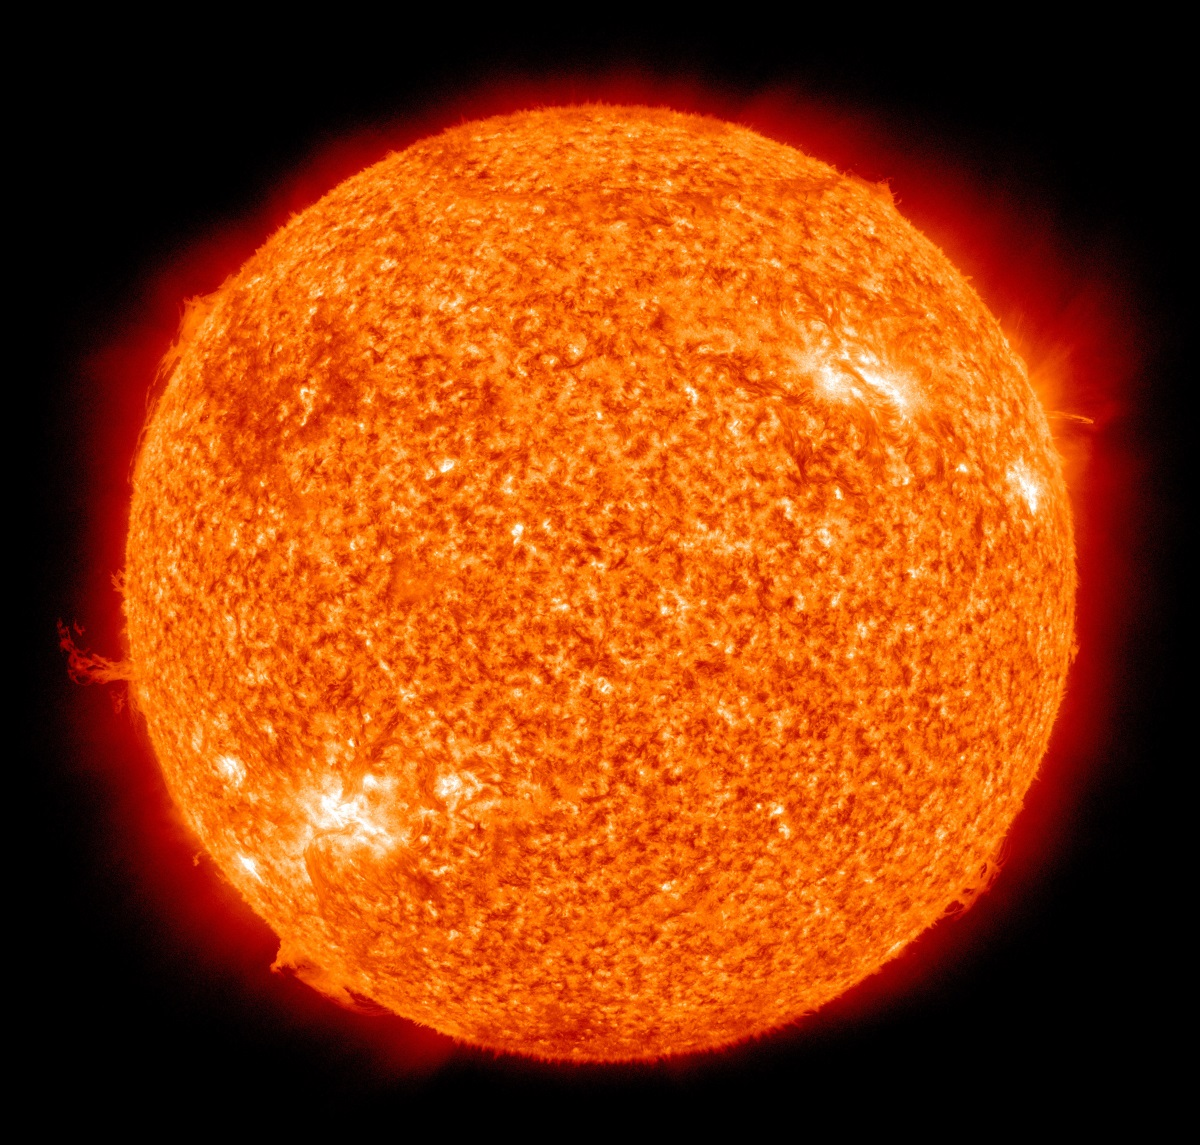
\includegraphics[scale=0.6]{media/NASA-Sun.jpg}
\column{0.5\textwidth}
{\small
\textcolor{yellow}{\bf Velkommen til del 3C! I denne delen av kurset skal du lære å regne på kjernereaksjoner. Du skal finne ut hvordan vi, basert på temperatur, tetthet og sammensetningen av kjernen til en stjerne kan beregne dens luminositet. Dette notatet tar normalt ca. en dobbelttime fysisk forelesning.}\\
\textcolor{yellow}{(Illustrasjon: NASA)}}
\hyperlink{intro2}{\pagebutton{Neste side}}
\end{columns}
\end{frame}
}


\begin{frame}
\label{intro2}
\lastpagebutton{feil_intro}{\bf SIDE 1/1/47}\\
\begin{alertblock}{Vi begynner som vanlig...}
...med litt brainstorming. Som det er {\bf svært viktig} at du gjør før du går videre.
\end{alertblock}
\href{https://nettskjema.no/a/167463}{\begin{minipage}{5cm}Trykk her for å varme opp\end{minipage}}\\
Er du klar og har sendt inn skjemaet?
\href{https://nettskjema.no/a/167463}{\choicebutton{Nei}}\ \ \ \ \hyperlink{blue_nytema1}{\choicebutton{Ja}}\\
\end{frame}





\renewcommand{\headline}{Kjernemasser}
{
\setbeamercolor{background canvas}{bg=blue}
\begin{frame}
\label{blue_nytema1}
\hyperlink{intro2}{\pagebutton{\small Forrige side}}
\nytemaside{fusjon}
\hyperlink{mass1}{\pagebutton{La oss se hva atomkjernenes masse har å gjøre med dette?}}
\end{frame}
}


\begin{frame}
\label{mass1}
\dlastpagebutton{intro2}{\bf SIDE 2/13/47}\\
{\Large
Du vet sannsynligvis allerede at det som produserer energien i de fleste stjerner er at 4 hydrogenkjerner (som består av et proton hver), smelter sammen til en heliumkjerne (som består av 2 protoner og 2 nøytroner). Men hvorfor blir det skapt energi når disse kjernene slåes sammen?
}
\hyperlink{mass2}{\pagebutton{Jeg har tenkt litt på dette nå og tror jeg har et svar...}}
\end{frame}



\begin{frame}
\label{mass2}
\lastpagebutton{mass1}{\bf SIDE 3/13/47}\\
{\Large
AhA! Opplagt! Vi ser at 2 av protonene her blir omgjort til nøytroner som har mindre masse enn protoner, og denne masseforskjellen blir omgjort til energi via Einsteins uttrykk $E=mc^2$ (som vi kommer tilbake til og skal utlede senere i kurset) \\
}
\hyperlink{feil_mass2f}{\choicebutton{Ja, selvsagt, den kjøper jeg!}}\\
\hyperlink{riktig_mass2r}{\choicebutton{Nei, jeg tror ikke det kan stemme!}}\\
\end{frame}


{
\setbeamercolor{background canvas}{bg=black}
\begin{frame}
\label{feil_mass2f}
\lastpagebutton{mass2}{\bf SIDE 4/13/47}\\
{\Large
\textcolor{yellow}{\Huge Er du såååå lettlurt enda? Har du ikke lært å ane fellene etter så mange interaktive forelesningsnotater? Nøytronene er jo selvfølgelig {\bf tyngre} enn protonene, de {\bf trenger} energi for å dannes!}
}
\hyperlink{mass3}{\pagebutton{Neste side}}
\end{frame}
}


{
\setbeamercolor{background canvas}{bg=yellow}
\begin{frame}
\label{riktig_mass2r}
\clastpagebutton{mass2}{\bf SIDE 5/13/47}\\
{\Large
Deg var det jammen ikke lett å lure i en felle! Du har vel kanskje begynt å ane fellene før de kommer? Du har helt rett, her var det noe galt! Nøytronene er jo selvfølgelig {\bf tyngre} enn protonene, de {\bf trenger} energi for å dannes!
}
\hyperlink{mass3}{\pagebutton{Neste side}}
\end{frame}
}




\begin{frame}
\label{mass3}
\lastpagebutton{mass2}{\bf SIDE 6/13/47}\\
{\Large
EEEhhhmmmmmm, OK? Heliumkjernen består av partikler som veier {\bf mer} enn i de 4 hydrogenkjernene til sammen. Likevel {\bf skapes} det energi i fusjonen? Hvor kommer denne fra?
}
\hyperlink{mass4}{\pagebutton{Tja...}}
\end{frame}


\begin{frame}
\label{mass4}
\lastpagebutton{mass3}{\bf SIDE 7/13/47}\\
La oss putte noen atomkjerner på kjøkkenvekta vår:
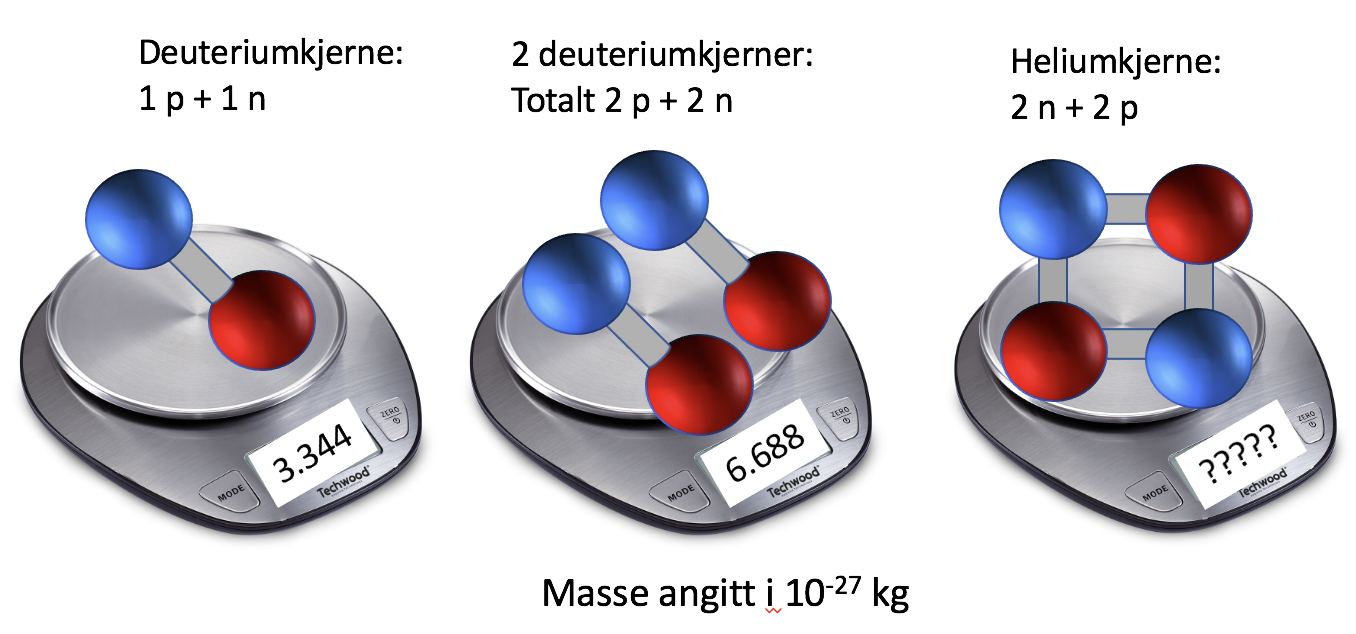
\includegraphics[scale=0.4]{media/atom_scale1.png}\\
Hadde bare noen rester i kjøleskapet, et par deuteriumkjerner og en heliumkjerne, det får duge! Deuterium er en isotop av hydrogen som har et proton og et nøytron i kjernen. Først måler vi en deuteriumkjerne, deretter to sammen og til slutt en heliumkjerne som består av nøyaktig det samme som to deuteriumkjerner.
\hyperlink{mass5}{\pagebutton{Hva tror du den siste vekte viser?}}
\end{frame}



\begin{frame}
\label{mass5}
\lastpagebutton{mass4}{\bf SIDE 8/13/47}\\
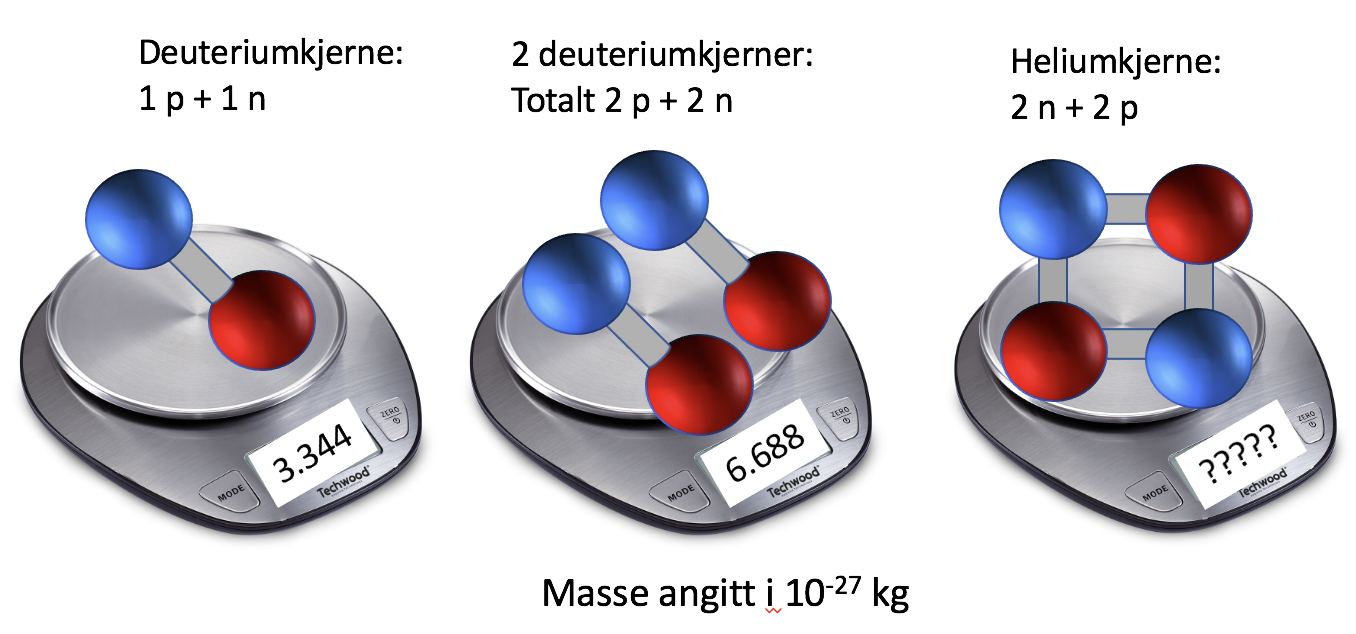
\includegraphics[scale=0.4]{media/atom_scale1.png}\\
Er det\\
\hyperlink{mass6}{\choicebutton{6.688}}\\
\hyperlink{mass6}{\choicebutton{mer enn 6.688}}\\
\hyperlink{mass6}{\choicebutton{mindre enn 6.688}}\\
\end{frame}


\begin{frame}
\label{mass6}
\lastpagebutton{mass5}{\bf SIDE 9/13/47}\\
{\bf\Large OG svaret er:}
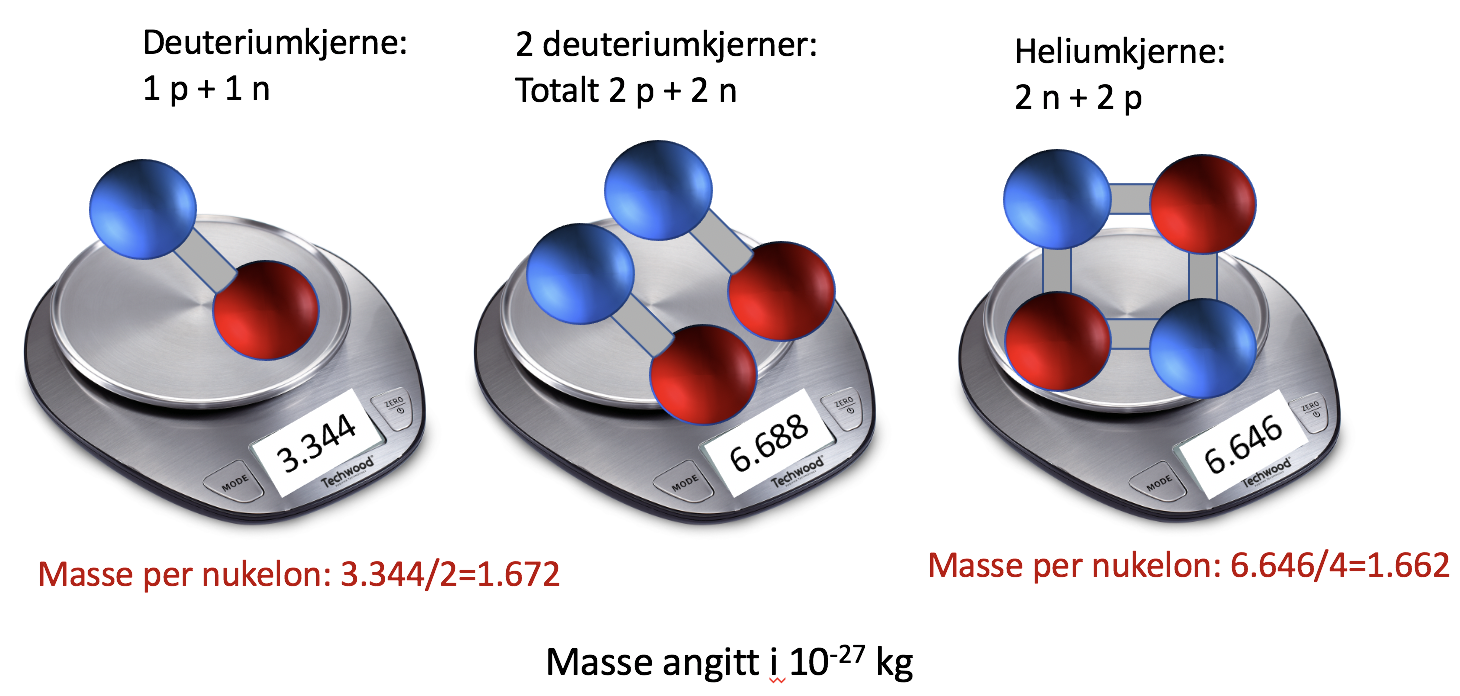
\includegraphics[scale=0.4]{media/atom_scale2.png}\\
Hæææææ! Vi har nøyaktig de samme partiklene på den midterste og siste vekt, likevel veier de forskjellig? Nøyaktig hvorfor skal vi komme tilbake til i relativitetsteorien i del 2. Men i relativitetsteori så er energi inkludert i masseregnskapet, energi som kinetisk og potensiell bidrar til masse. {\bf Dermed er masse ikke en additiv størrelse i relativitetsteori.}
\hyperlink{mass7}{\pagebutton{Neste side}}
\end{frame}

\begin{frame}
\label{mass7}
\lastpagebutton{mass6}{\bf SIDE 10/13/47}\\
{\bf\Large OG svaret er:}
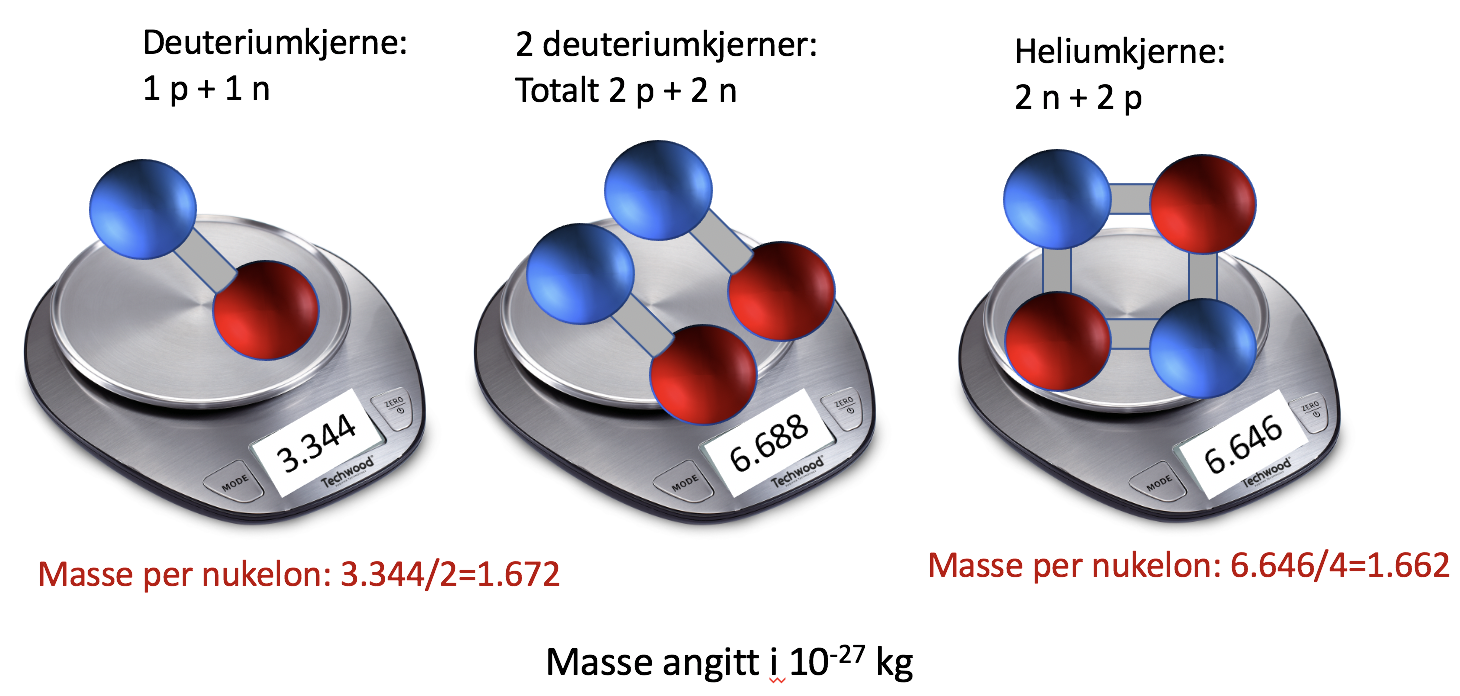
\includegraphics[scale=0.4]{media/atom_scale2.png}\\
Det er ingen enkel sammenheng mellom hvilke og hvor mange kjernepartikler vi har og massen til atomkjernen, det avhenger bl.a. av bindingsenergier (sterk kjernekraft) i atomkjernen. Det enkleste vi kan gjør er å snakke om {\bf masse per nukleon}, dvs. vi tar totalmassen og deler på antall nukleoner (=protoner og nøytroner). Da får vi et mål for midlere masse til en kjernepartikkel.
\hyperlink{mass8}{\pagebutton{Neste side}}
\end{frame}

\begin{frame}
\label{mass8}
\lastpagebutton{mass7}{\bf SIDE 11/13/47}\\
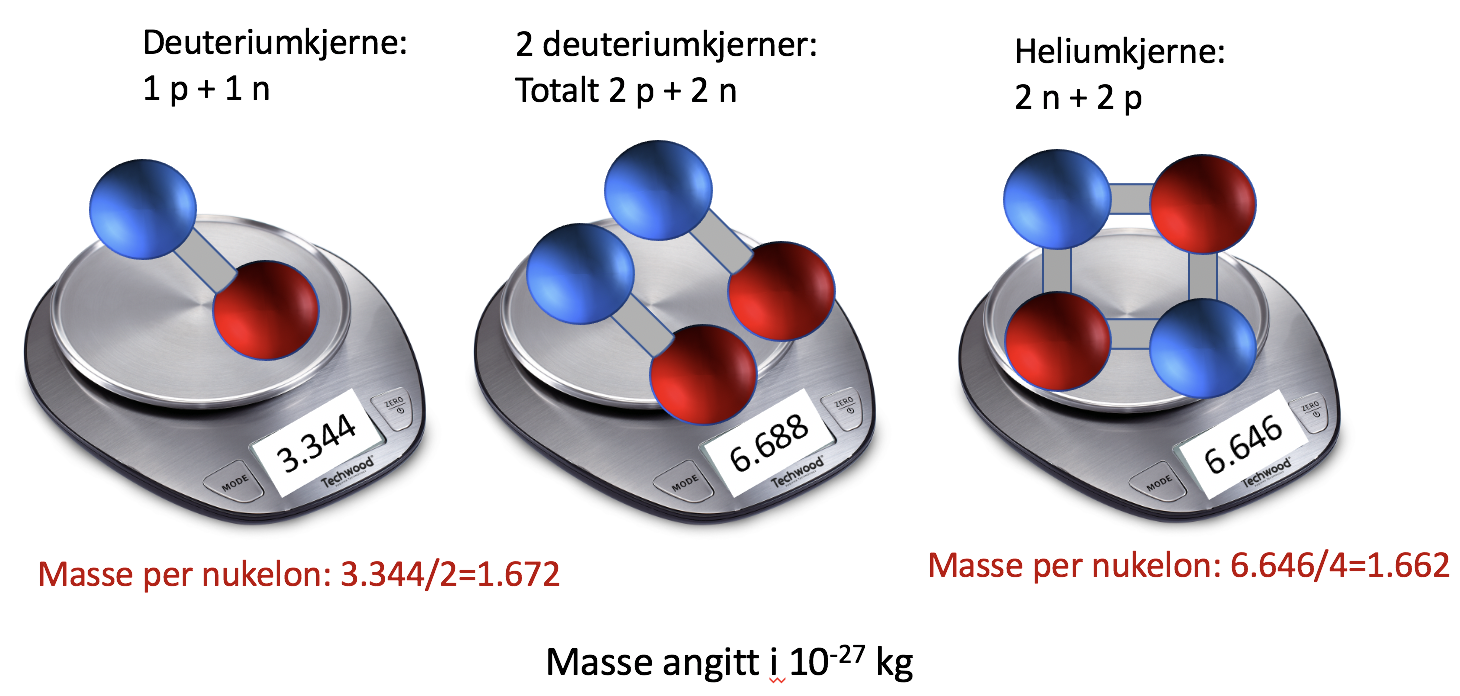
\includegraphics[scale=0.4]{media/atom_scale2.png}\\
Vi ser av figuren at midlere masse per atomkjerne altså er mindre i helimkjernen enn i deuteriumkjernen. Det betyr at hvis vi hadde klart å fusjonere to deuteriumkjerner til en heliumkjerne så ville vi fått energi til overs, denne overflødige massen ville blitt omgjort til energi (kinetisk og/eller stråling). For å vite om energi frigjøres i en kjernereasjon (fusjon eller fisjon) så må vi altså se på masse per nukleon før og etter prosessen. Er den mindre etter blir det frigjort energi.
\hyperlink{mass9}{\pagebutton{Neste side}}
\end{frame}

\begin{frame}
\label{mass9}
\lastpagebutton{mass8}{\bf SIDE 12/13/47}\\
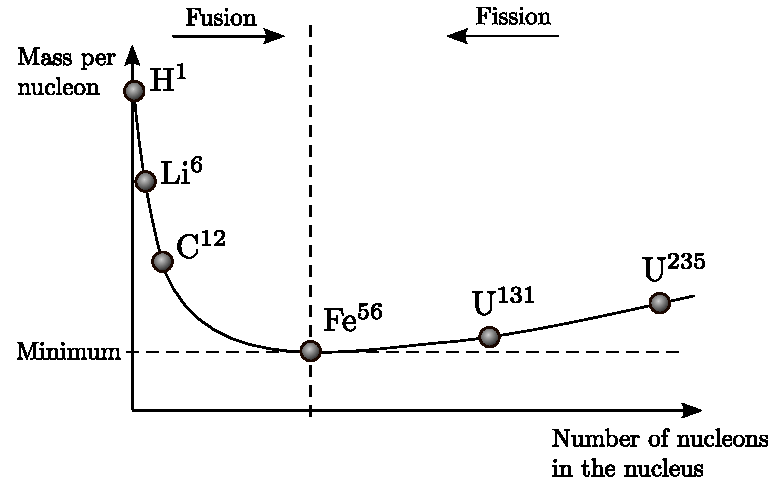
\includegraphics[scale=0.6]{media/fig_19-3.pdf}\\
Figuren viser en skisse av grafen for nukleontall (antall nukleoner i en atomkjerne) på x-aksen og masse per nukleon på y-akse. {\bf Vi ser at masse per nukleon faller kraftig fra Hydrogen og til tyngre grunnstoffer. Men kun frem til jern (Fe). Deretter øker massen per nukleon igjen til de tyngde grunnstoffene.} \textcolor{red}{Vi vil altså vinne energi hvis vi går fra høy til lav masse per nukleon! Altså hvis vi fusjonerer en lett atomkjerne, eller fisjonerer en tung atomskjerne.}
\hyperlink{mass10}{\pagebutton{Neste side}}
\end{frame}

\begin{frame}
\label{mass10}
\lastpagebutton{mass9}{\bf SIDE 13/13/47}\\
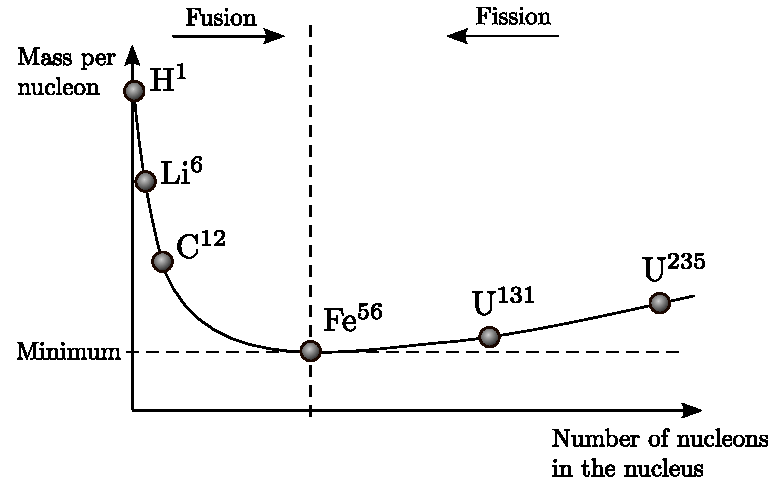
\includegraphics[scale=0.6]{media/fig_19-3.pdf}\\
Prosesser som krever energi er svært vanskelig å få til. Dvs. at det er svært vanskelig å fusjonere grunnstoffer fra jern og oppover til enda tyngde grunnstoffer (hvordan har da disse oppstått i universet? Dette kommer vi tilbake til). På samme måte er det svært vanskelig å fisjonere lette grunnstoffer. {\bf Men det viktigste nå er å se at man skaper energi ved fusjon av de letteste grunnstoffene som hydrogen!}
\hyperlink{blue_nytema2}{\pagebutton{Neste side}}
\end{frame}


\renewcommand{\headline}{Fusjon}
{
\setbeamercolor{background canvas}{bg=blue}
\begin{frame}
\label{blue_nytema2}
\hyperlink{mass10}{\pagebutton{\small Forrige side}}
\nytemaside{reaksjoner}
\hyperlink{fusj1}{\pagebutton{Hva skal til for å starte fusjon da?}}
\end{frame}
}


\begin{frame}
\label{fusj1}
\lastpagebutton{mass10}\label{fusjon}{\bf SIDE 14/24/47}\\
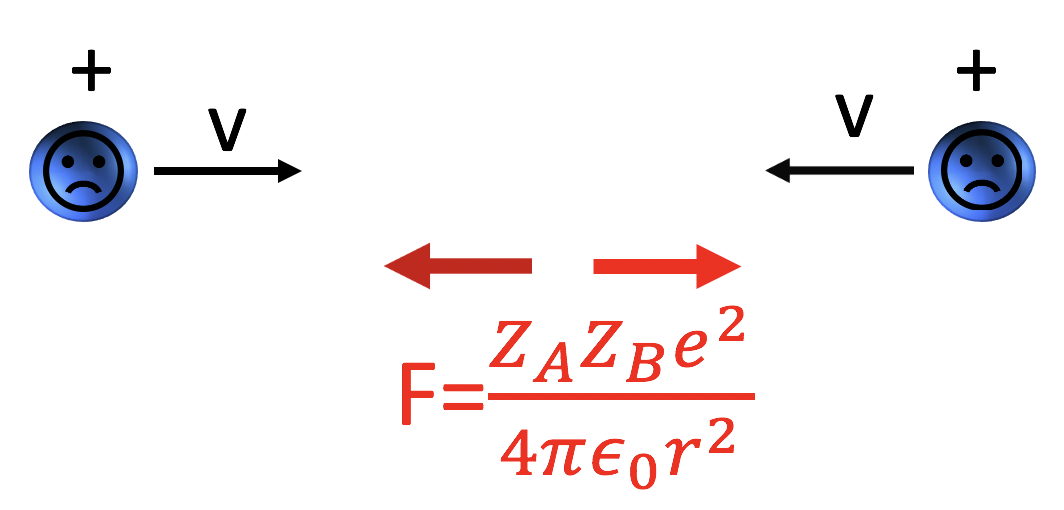
\includegraphics[scale=0.6]{media/approaching_protons.png}\\
Her ser vi to protoner (hydrogenkjerner) som er på vei mot hverandre i full fart. {\bf Men vil de kunne fusjonere?} I midten ser vi Coulombkraften. Den blir jo sterkere og sterkere jo nærmere de kommer og går mot uendelig sterk når $r\rightarrow0$. {\bf Så hvordan får vi til fusjon i det hele tatt? Vil ikke Coulombkrafta stoppe ethvert forsøk?} Tenk deg godt om før du går videre, hvordan kommer protonene nær hverandre så de kan fusjonere?
\hyperlink{fusj2}{\pagebutton{\small Hmmmmm.....jeg har tenkt godt etter...}}
\end{frame}

\begin{frame}
\label{fusj2}
\lastpagebutton{fusj1}{\bf SIDE 15/24/47}\\
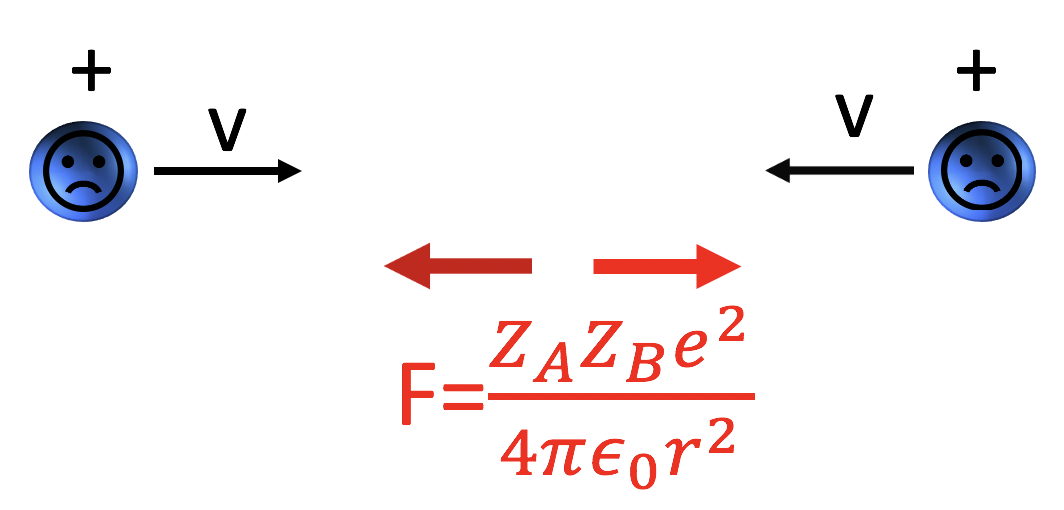
\includegraphics[scale=0.6]{media/approaching_protons.png}\\
Når du har tenkt deg godt om, ta nå en titt på \href{https://www.uio.no/studier/emner/matnat/astro/AST2000/h20/undervisningsmateriell/interaktive-forelesningsnotater/3c/videoer/video3c_1.mp4}{denne videoen her} som forklarer dette og mer til.
\hyperlink{fusj3}{\pagebutton{Jeg har sett videoen!}}
\end{frame}


\begin{frame}
\label{fusj3}
\lastpagebutton{fusj2}{\bf SIDE 16/24/47}\\
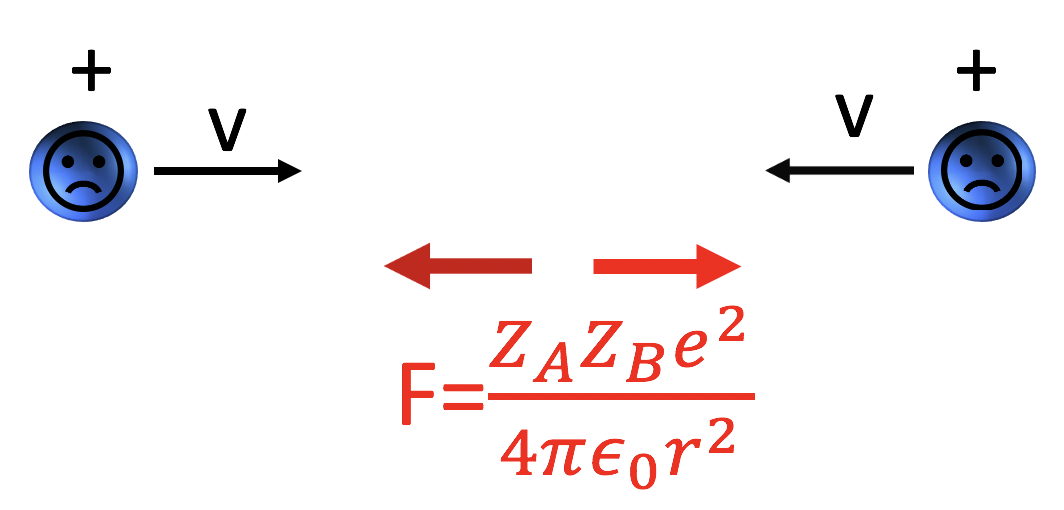
\includegraphics[scale=0.6]{media/approaching_protons.png}\\
Hvis du slet med å forstå videoen, spør foreleser! Vi ser altså at kvanteeffekter og tilfeldigheter er viktige for å vite om vi får en fusjon ved en nærpassering av atomkjerner eller ikke. Et mål som brukes på dette er det såkalte {\bf kollisjonstverrsnittet}. Dette er en abstrakt størrelse som gjør regningen med slike kvantetilfeldigheter enklere.
\hyperlink{fusj4}{\pagebutton{Neste side}}
\end{frame}


\begin{frame}
\label{fusj4}
\lastpagebutton{fusj3}{\bf SIDE 17/24/47}\\
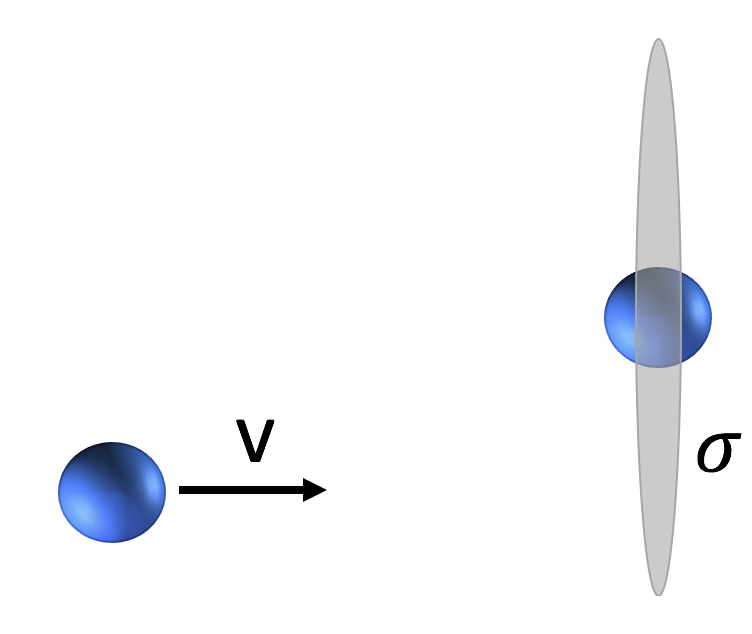
\includegraphics[scale=0.4]{media/cross_section.png}\\
Tenk deg at du ser kollisjonen fra det ene protonets hvilesystem. Da ser vi for oss at dette protonet spenner ut en skive med areal $\sigma$. Dette er det såkalte tverrsnittet. Hvis det andre protonet kommer innenfor denne skiven, blir det fusjon, hvis ikke, blir det ingen fusjon. \textcolor{red}{Merk at det ikke er dette som faktisk skjer!} Det er kun en måte å regne med kvantetilfeldighetene på. Det vi ser her er at jo større kollisjonstverrsnitt, jo større sannsynlighet for fusjon. I AST2000 skal du kun ha hørt om begrepet som du kommer til å treffe mye senere i fysikkstudiet.
\hyperlink{fusj5}{\pagebutton{Neste side}}
\end{frame}

\begin{frame}
\label{fusj5}
\lastpagebutton{fusj4}{\bf SIDE 18/24/47}\\
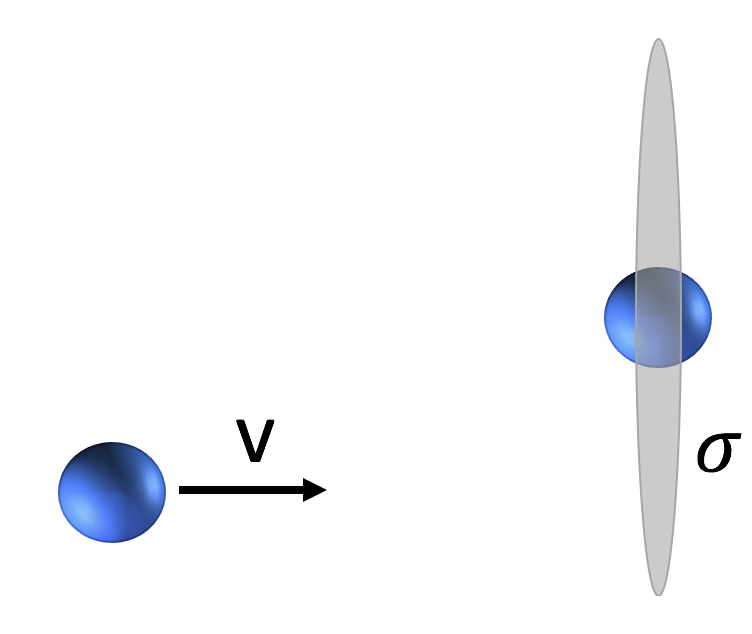
\includegraphics[scale=0.4]{media/cross_section.png}\\
Hvis du er interessert, så kan du i \href{https://www.uio.no/studier/emner/matnat/astro/AST2000/h20/undervisningsmateriell/lecture_notes/part3c.pdf}{de vanlige forelesningsnotatene} i avsnitt 3.1 lese et eksempel om hvordan du bruker dette tverrsnittet for å beregne fusjonsrater, men dette er som sagt {\bf ikke pensum}. Hver fusjonsreaksjon har sitt tverrsnitt-areal, men å beregne disse arealene krever kompliserte kvantemekaniske regninger og ofte er de for kompliserte til å kunne løses og man må ty til eksperimenter for å finne dem.
\hyperlink{fusj6}{\pagebutton{Neste side}}
\end{frame}

\begin{frame}
\label{fusj6}
\lastpagebutton{fusj5}{\bf SIDE 19/24/47}\\
\begin{columns}
\column{0.5\textwidth}
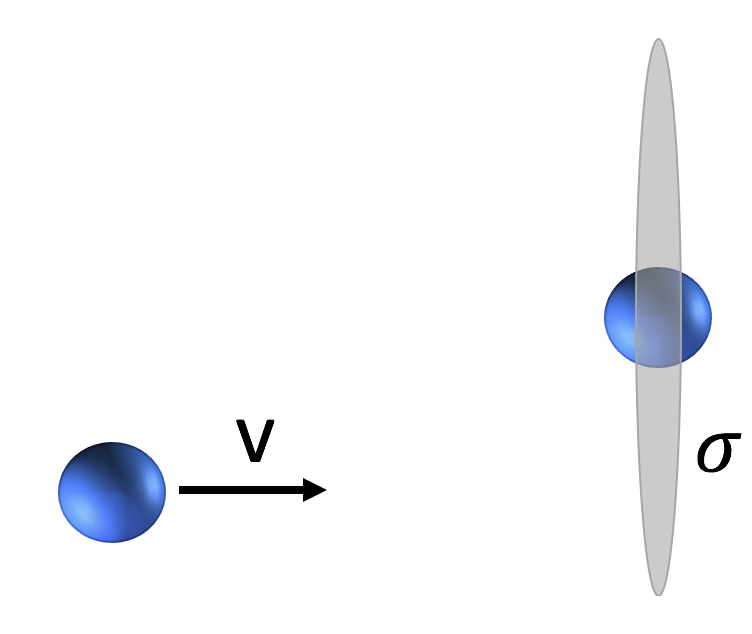
\includegraphics[scale=0.4]{media/cross_section.png}\\
Resultatet av regning av fusjonsrater med slike tverrsnitt gir oss et uttrykk for energiproduksjon per tid gitt tetthet, sammensetning og temperatur, {\bf for en gitt fusjonsprosess}.
\column{0.5\textwidth}
Den kan tilnærmes som:
\[
\epsilon_{AB}=\epsilon_{0,AB}X_AX_B\rho^\alpha T^\beta
\]
der $\epsilon_{AB}$ er energi per tid per kg gass som frigjøres av fusjonsreaksjoner mellom kjerner av type $A$ og $B$. $\epsilon_{0,AB}$ er en konstant som avhenger av fusjonen, $X_A$ og $X_B$ er masseforhold av atomkjernene $A$ og $B$, $\rho$ er tettheten av gassen og $T$ er temperaturen til gassen. Eksponentene $\alpha$ og $\beta$ avhenger av hvilken fusjon (hvilke kjerner) vi ser på.
\hyperlink{fusj7}{\pagebutton{Neste side}}
\end{columns}
\end{frame}


\begin{frame}
\label{fusj7}
\lastpagebutton{fusj6}{\bf SIDE 20/24/47}\\
\begin{columns}
\column{0.5\textwidth}
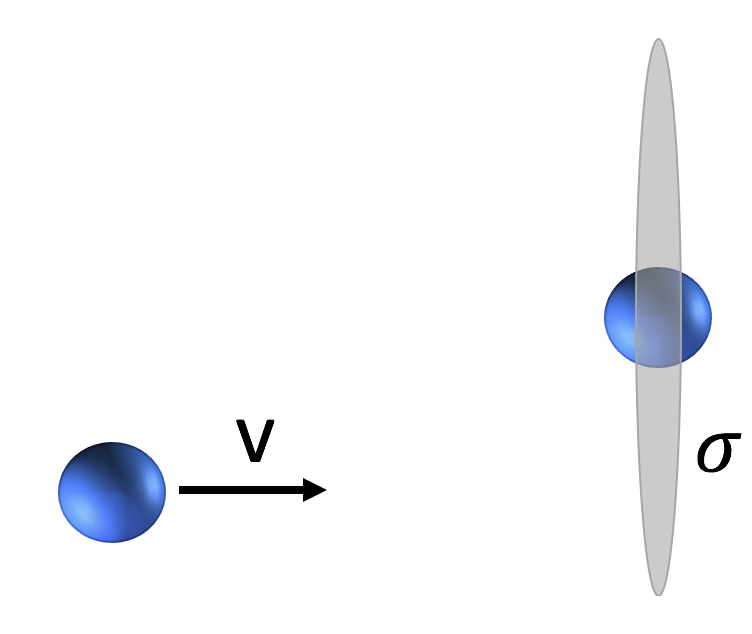
\includegraphics[scale=0.4]{media/cross_section.png}\\
{\bf\Large
\[
\epsilon_{AB}=\epsilon_{0,AB}X_AX_B\rho^\alpha T^\beta
\]
}
\column{0.5\textwidth}
{\bf Masseforholdene $X_A$ og $X_B$} er andelen av massen av gassen som tilsvarer $A$ og $B$-kjerner:
\[
X_A=\frac{n_Am_A}{n\mu m_H}
\]
der $n_A$ er antall $A$-kjerner per volum (antalltetthet), $m_A$ er massen til kjerne A, $n$ er total antalltetthet til gassen, altså totalt antall gasspartikler (av alle typer) per volum og $\mu m_H$ er midlere masse til en gasspartikkel. Vi ser at vi over brøkstreken har den totale masse i $A$-kjerner per volum mens vi under brøkstreken har total gassmasse per volum, altså vanlig massetettet $\rho$.
\hyperlink{fusj8}{\pagebutton{Neste side}}
\end{columns}
\end{frame}


\begin{frame}
\label{fusj8}
\lastpagebutton{fusj7}{\bf SIDE 21/24/47}\\
\begin{columns}
\column{0.5\textwidth}
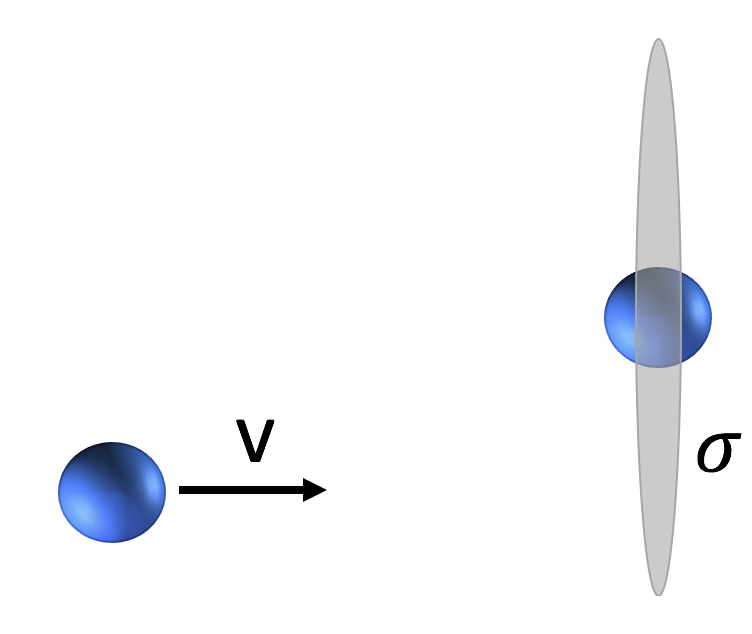
\includegraphics[scale=0.4]{media/cross_section.png}\\
{\bf\Large
\[
\epsilon_{AB}=\epsilon_{0,AB}X_AX_B\rho^\alpha T^\beta
\]
}
\column{0.5\textwidth}
Merk at denne formelen er en tilnærmelse som er gyldig innenfor visse temperaturområder, dette blir alltid oppgitt med uttrykket. I det neste nå skal vi se på 3 av de mest aktuelle kjernereaksjonene i stjerner og hvordan dette uttrykket ser ut i de forskjellige tilfellene. For å forstå litt mer av denne formelen, ta en titt på \href{https://www.uio.no/studier/emner/matnat/astro/AST2000/h20/undervisningsmateriell/interaktive-forelesningsnotater/3c/videoer/video3c_2.mp4}{denne videoen her}
\hyperlink{fusj9}{\pagebutton{Neste side}}
\end{columns}
\end{frame}

\begin{frame}
\label{fusj9}
\lastpagebutton{fusj8}{\bf SIDE 22/24/47}\\
\[
\epsilon_{AB}=\epsilon_{0,AB}X_AX_B\rho^\alpha T^\beta
\]
Som sagt, så er $\epsilon_{AB}$ energiproduksjon per tid per masse, altså per kg av gassen. Det blir vel luminositet per kg av gassen? Eller
\[
\frac{dL}{dm}=\sum_{AB}\epsilon_{AB}
\]
der vi summer over alle mulige kjernereaksjoner som kan foregå i stjernen. Dette er en sammenheng som er svært viktig når man modellerer stjerner. Da antar man ofte at temperatur og tetthet er den samme for en gitt $r$, altså at vi har kulesymmetri. Dermed har vi også at luminositeten som produseres $L(r)$ og $\epsilon(r)=\sum_{AB}\epsilon_{AB}(r)$ er en funksjon kun av $r$. Hvilke av de følgende likninger vil da beskrive energiproduksjonen som funksjon av $r$:
\hyperlink{feil_fusj9f}{\choicebutton{$\frac{d\epsilon(r)}{dr}=\frac{\rho(r)L(r)}{4\pi r^2}$}}\ \ \ \hyperlink{feil_fusj9f}{\choicebutton{$\frac{d\epsilon(r)}{dr}=\frac{4\pi r^2L(r)}{\rho(r)}$}}\hyperlink{feil_fusj9f}{\choicebutton{$\frac{dL(r)}{dr}=\frac{\rho(r)\epsilon(r)}{4\pi r^2}$}}\ \ \ \hyperlink{feil_fusj9f}{\choicebutton{$\frac{dL(r)}{dr}=\frac{4\pi r^2\epsilon(r)}{\rho(r)}$}}\ \ \ \hyperlink{riktig_fusj9r}{\choicebutton{$\frac{dL(r)}{dr}=4\pi r^2\rho(r)\epsilon(r)$}}
\end{frame}



{
\setbeamercolor{background canvas}{bg=black}
\begin{frame}
\label{feil_fusj9f}
\lastpagebutton{fusj9}{\bf SIDE 23/24/47}\\
{\Large
\textcolor{yellow}{\Huge Det ble galt! Hva er volumet av et infinitesimalt lite kuleskall i avstand $r$ med tykkelse $dr$? Og hva blir massen $dm$ av dette kuleskallet? Kan du sette inn for $dm$ i den ene formelen på forrige side?}
}
\end{frame}
}


{
\setbeamercolor{background canvas}{bg=yellow}
\begin{frame}
\label{riktig_fusj9r}
\clastpagebutton{fusj9}{\bf SIDE 24/24/47}\\
{\Large
Massen av kuleskallet i avstand $r$ med tykkelse $dr$ blir vel:
\[
dm=4\pi r^2\rho(r)dr
\]
Setter vi det inn i
\[
\frac{dL(r)}{dm}=\epsilon(r)
\]
så får vi differensiallikningen
\[
\frac{dL(r)}{dr}=4\pi r^2\rho(r)\epsilon(r)
\]
Dette er enda en av likningene som løses sammen med bl.a. likningen for hydrostatisk likevekt når man modellerer en stjerne. Ved å løse dette settet med 4-5 koblede differensiallikninger i $r$ kan man finne bl.a. $\rho(r)$ og $T(r)$ i stjerna. Veldig mye av det man vet om stjerner idag er bygget på slike modeller der man utvikler stjerner over tid i modellen.
}
\hyperlink{pause}{\pagebutton{Neste side}}
\end{frame}
}



{
\setbeamercolor{background canvas}{bg=cyan}
\begin{frame}
\label{pause}
\hyperlink{riktig_fusj9r}{\pagebutton{\small Forrige side}}
{\Huge
\centerline{Kaffe?}
\centerline{
\includegraphics[scale=4]{media/drink-coffee.png}}\\
En strekk på beina! Litt frisk luft! Og er du heldig kan du nyte varmen fra solas fusjonsreaksjoner i ansiktet.
\vspace*{0.5cm}
Ikke lov å fortsette før du har tatt minst 15 min. pause!
}\\
\vspace*{0.5cm}
\hyperlink{blue_nytema3}{\pagebutton{La oss regne litt på fusjonsreaksjoner!}}
\end{frame}
}

\renewcommand{\headline}{Fusjonsreaksjonene}
{
\setbeamercolor{background canvas}{bg=blue}
\begin{frame}
\label{blue_nytema3}
\hyperlink{riktig_fusj9r}{\pagebutton{\small Forrige side}}
\nytemaside{snp}
\hyperlink{reak1}{\pagebutton{Sett igang!}}
\end{frame}
}


\begin{frame}
\label{reak1}
\lastpagebutton{riktig_fusj9r}\label{reaksjoner}{%\small{\bf SIDE 25/38/47}\\
I AST2000 skal vi se på 3 av de viktigste fusjonsreaksjonene som foregår i stjerner. I stjerner på hovedserie som er der stjernene tilbringer det meste av sitt liv, så {\bf fusjoners 4 hydrogenatomer (altså protoner) til en heliumkjerne (2 protoner og 2 nøytroner).} Dette skjer jo ikke i {\bf en} kollisjon, det er flere mellomsteg i denne reaksjonen. Det kan skje via 2 forskjellige slike reaksjonsrekke.
\begin{itemize}
\item Den ene heter {\bf proton-proton-kjeden} og den andre er
\item {\bf CNO-syklusen}. I den siste trengs det atomkjerner av karbon, nitrogen og oksygen (C, N og O) til stede som katalysatorer i prosessen.
\end{itemize}
Disse reaksjonene har ganske forskjellige temperaturavhengighet og temperaturen i kjernen til stjernen avgjør hvilke av disse reaksjonene som produserer mest energi. I stjerner som har brukt opp det meste av hydrogenet i sentrum så {\bf fusjoneres helium videre til karbon i trippel-alpha-prosessen} som vi også skal se på. Vi tar en og en etter tur...}
\hyperlink{reak2}{\pagebutton{Neste side}}
\end{frame}

\begin{frame}
\label{reak2}
\lastpagebutton{reak1}{\bf SIDE 26/38/47}\\
{\Large
I det følgende skal vi skrive fusjonsreaksjonslikninger med symboler \atom{A}{Z}{X} der $X$ er kjemisk symbol, $A$ er totalt antall nukleoner i kjernen (protoner + nøytroner) og $Z$ er antall protoner i kjernen. Dermed blir for eksempel deuterium som har et proton og et nøytron skrevet som \atom{2}{1}{H}.
}
\hyperlink{reak3}{\pagebutton{Neste side}}
\end{frame}



\begin{frame}
\label{reak3}
\lastpagebutton{reak2}{\bf SIDE 27/38/47}\\
\begin{block}{Proton-proton-kjeden (pp-kjeden)}
\begin{columns}
\column{0.7\textwidth}
Denne skjer ved hjelp av følgende reaksjoner:
\bua
{\hydrogen}+\hydrogen&\rightarrow&{\deuterium}+\positron+\neutrino \\
{\deuterium} +\hydrogen&\rightarrow&{\hethree}+\photon \\
{\hethree} +\hethree&\rightarrow&{\helium}+2\times\hydrogen
\eua
{\small (Illustrasjon: Wikipedia)}
\column{0.3\textwidth}
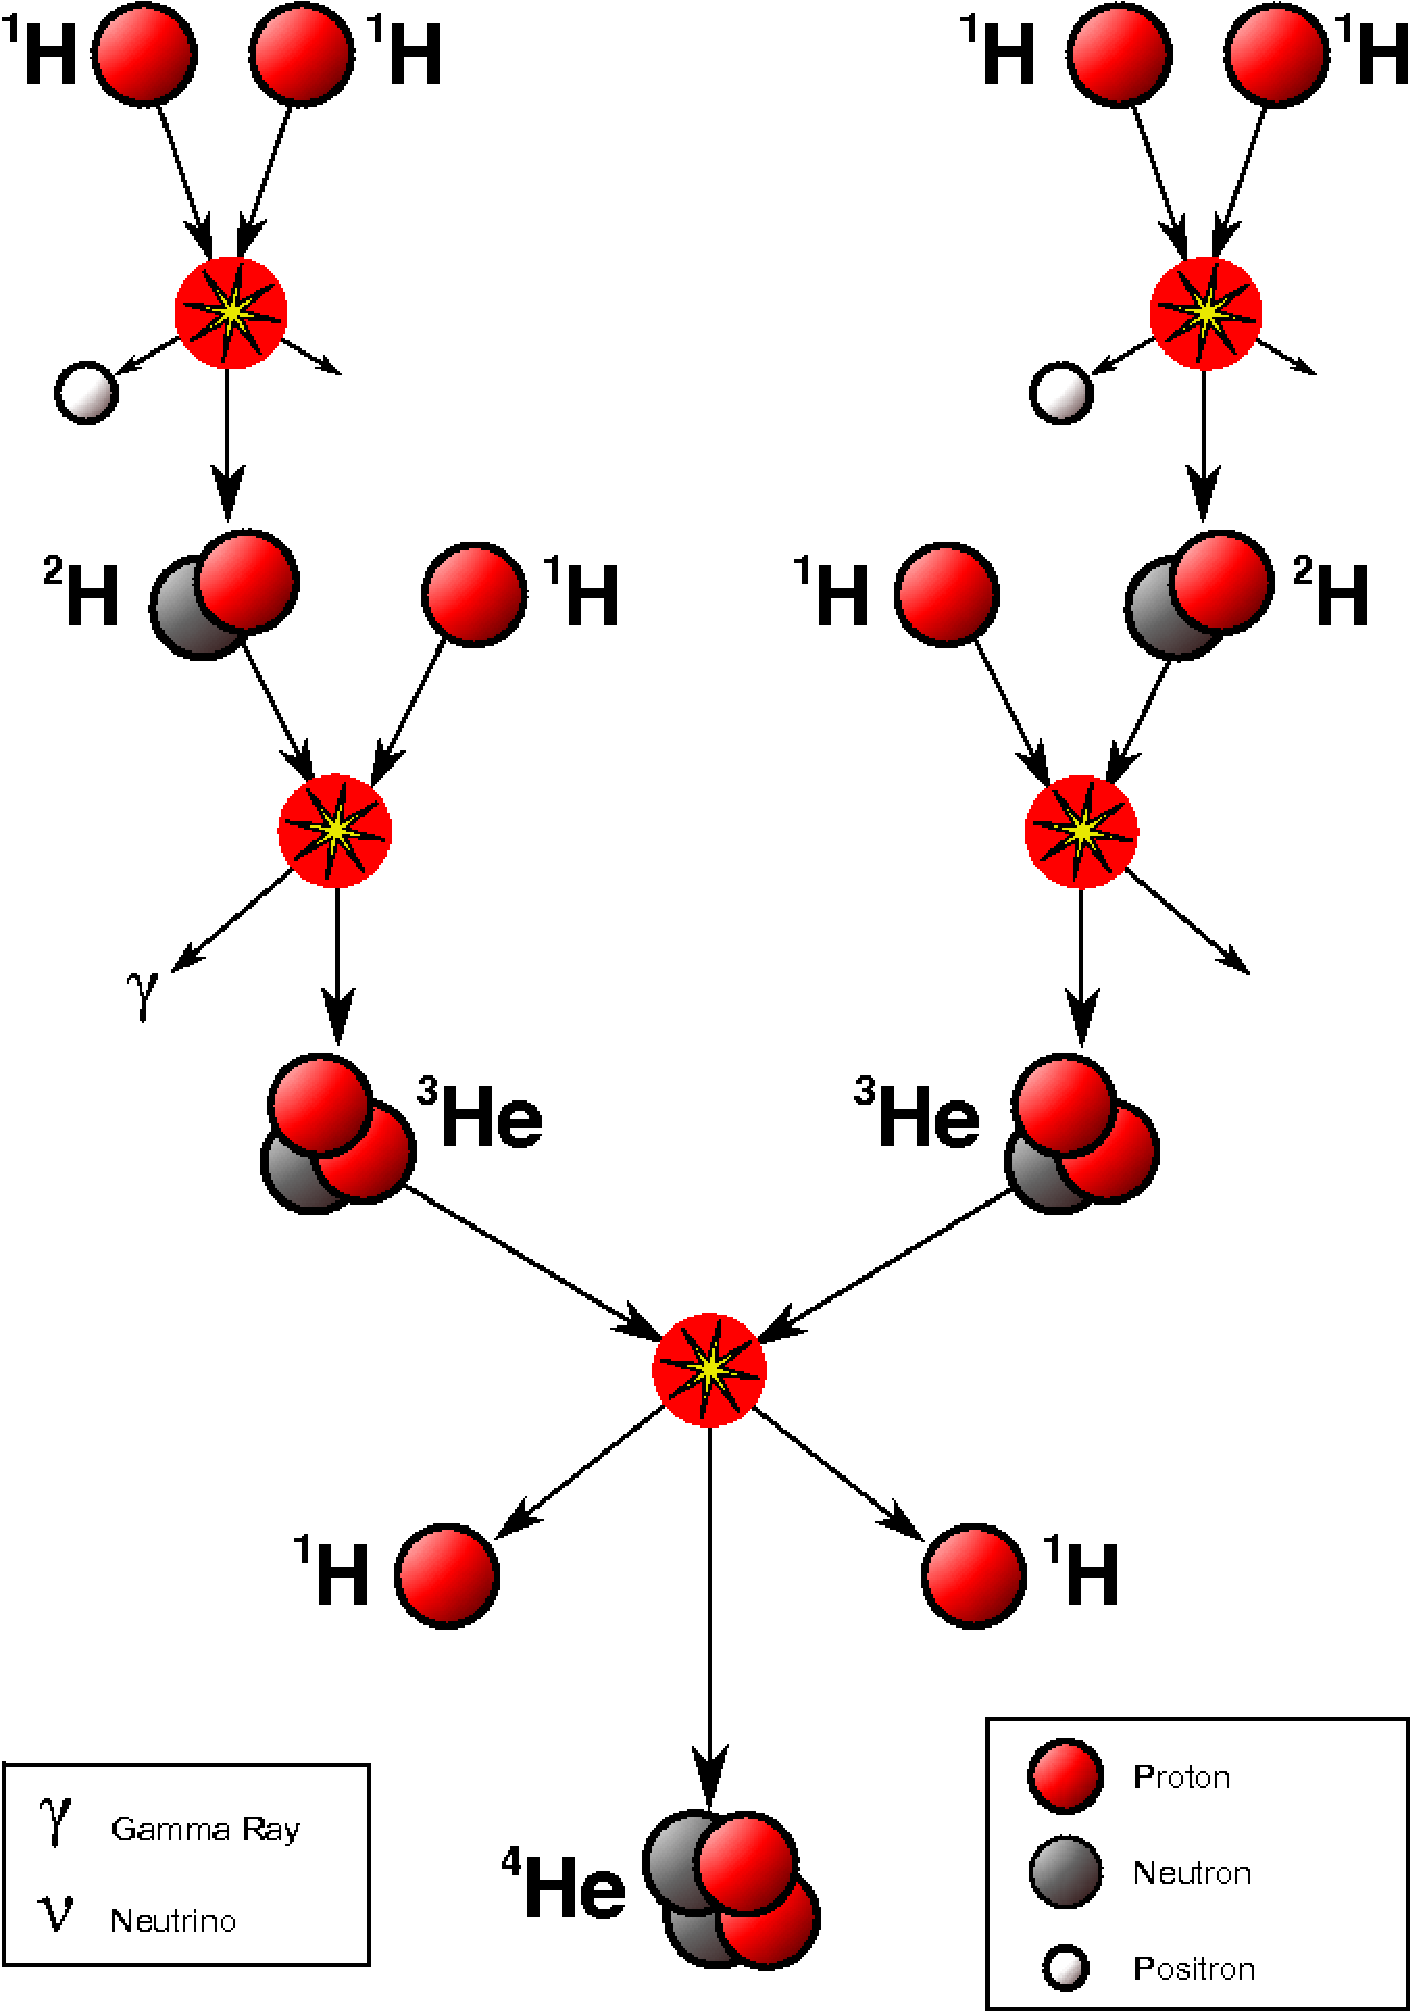
\includegraphics[scale=0.1]{media/pp_chain_Wiki.pdf}
\end{columns}
Her er $\positron$ et positron (anti-elektron), $\neutrino$ er et elektron-assosiert nøytrino og $\photon$ er et foton (energi). Reaksjonsraten til pp-kjeden er
\[
\varepsilon_{\rm pp}\approx\varepsilon_{\rm 0,pp}\,X_H^2\,\rho\, T_6^4,
\]
med
\[
\varepsilon_{\rm 0,pp}=1.08\times10^{-12}{\rm\ Wm^3/kg^2}
\]
\end{block}
{\bf Men hva betyr $T_6$????}
\hyperlink{reak4}{\pagebutton{Neste side}}
\end{frame}


\begin{frame}
\label{reak4}
\lastpagebutton{reak3}{\bf SIDE 28/38/47}\\
{\Large
Når man jobber med kjernereaksjoner så har vi normalt så høye temperaturer at vi letter skriving med å definere $T_X$ som temperaturen målt i $10^X$ Kelvin. Da blir f.eks.
\begin{itemize}
\item $T_6$ temperaturen målt i millioner Kelvin. For eksempel $T_6=2.5$ betyr at temperaturen er på $2.5\times10^6$\,K.
\item $T_8$ temperaturen målt i hundre millioner Kelvin. For eksempel $T_8=1.3$ betyr at temperaturen er på $1.3\times10^8$\,K.
\end{itemize}
Uttrykket for reaksjonsraten i pp-reaksjonen:
\[
\varepsilon_{\rm pp}\approx\varepsilon_{\rm 0,pp}\,X_H^2\,\rho\, T_6^4,
\]
er gyldig omkring $T_6\approx15$ som er der pp-reaksjonen normal er effektiv. Dette tilsvarer solas kjernetemperatur.
}
\hyperlink{reak5}{\pagebutton{Neste side}}
\end{frame}


\begin{frame}
\label{reak5}
\lastpagebutton{reak4}{\bf SIDE 29/38/47}\\
{\small
\begin{block}{CNO-syklusen}
\begin{columns}
\column{0.6\textwidth}
Denne skjer ved hjelp av følgende reaksjoner:
\bua
{\atom{12}{6}{C}} +\hydrogen&\rightarrow&{\atom{13}{7}{N}}+\photon \\
{\atom{13}{7}{N}}&\rightarrow&{\atom{13}{6}{C}}+\positron+\neutrino \\
{\atom{13}{6}{C}} +\hydrogen&\rightarrow&{\atom{14}{7}{N}}+\photon \\
{\atom{14}{7}{N}} +\hydrogen&\rightarrow&{\atom{15}{8}{O}}+\photon \\
{\atom{15}{8}{O}}&\rightarrow&{\atom{15}{7}{N}}+\positron+\neutrino \\
{\atom{15}{7}{N}} +\hydrogen&\rightarrow&{\atom{12}{6}{C}}+\helium
\eua\\
\vspace*{-0.3cm}{\footnotesize (Illustrasjon: Wikipedia)}
\column{0.4\textwidth}
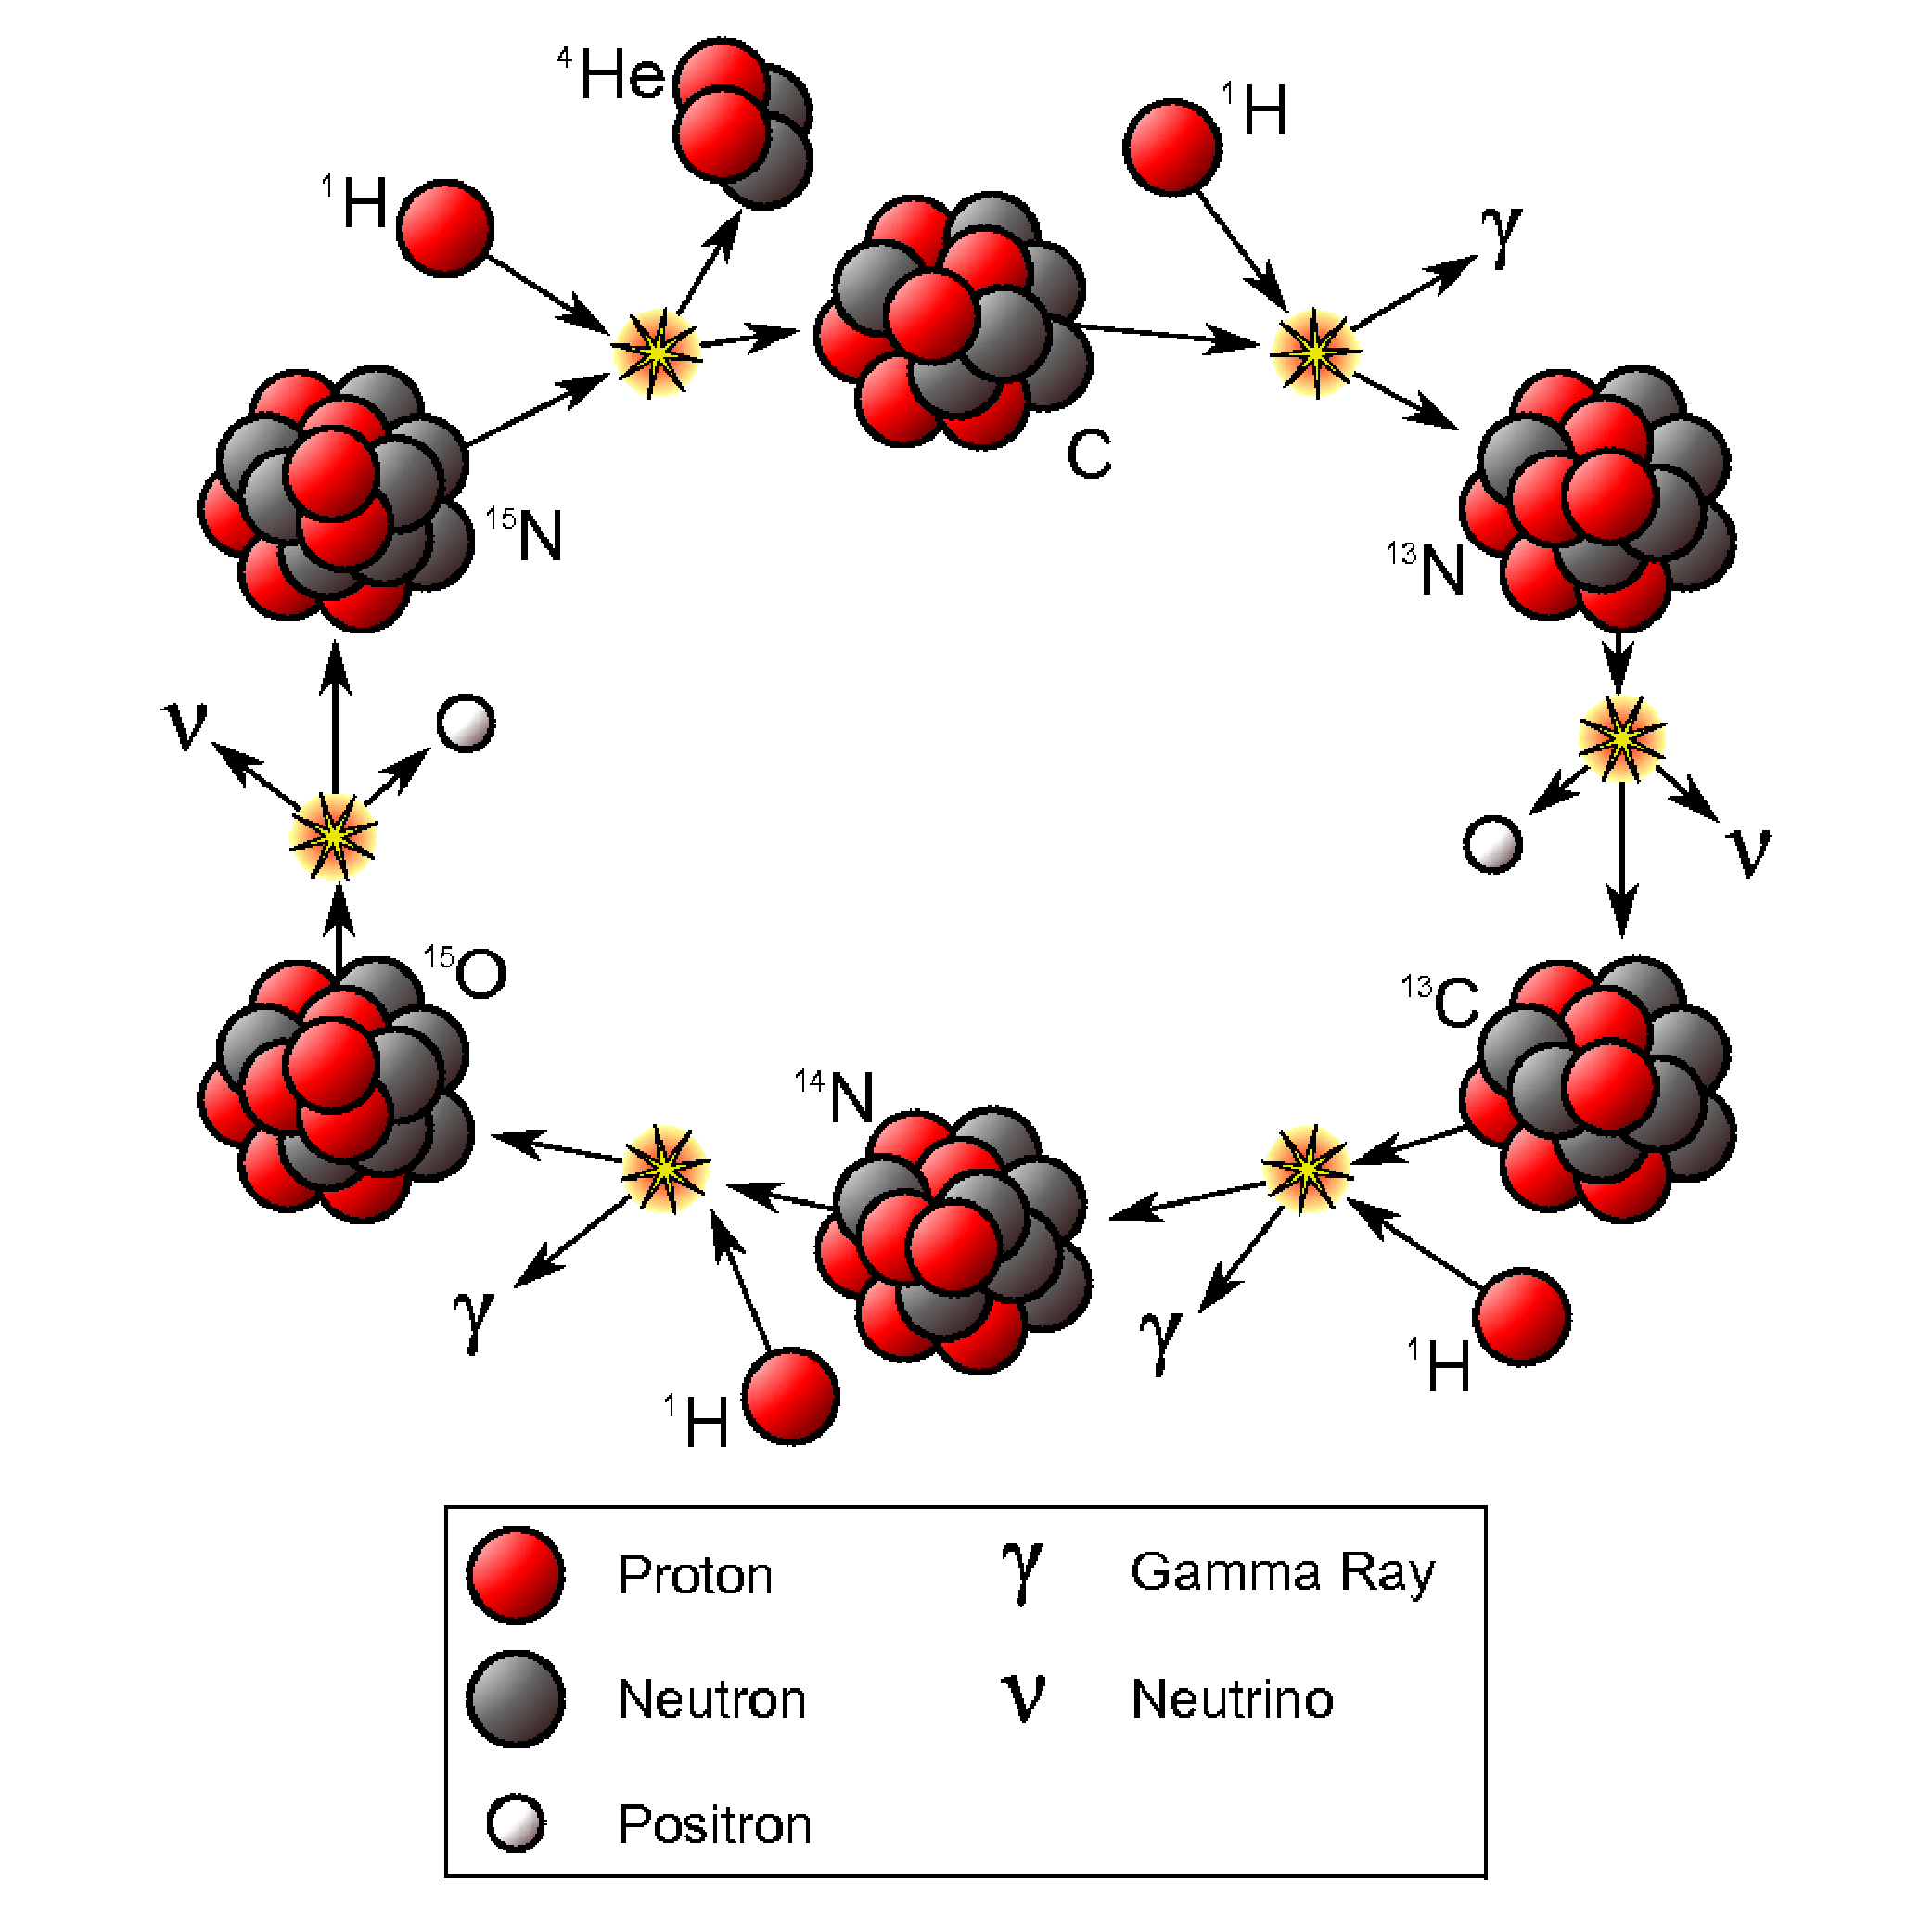
\includegraphics[scale=0.12]{media/CNO_cycle_Wiki.pdf}
\end{columns}
Og med
\[
\varepsilon_{\rm CNO}=\varepsilon_{0, {\rm CNO}}\;X_H\;X_{\rm CNO}\;\rho T_6^{20},
\]
hvor
\[
\varepsilon_{0, {\rm CNO}}=8.24\times10^{-31}{\rm\ Wm^3/kg^2}
\]
Her er $X_{\rm CNO}$ det totale masseforholdet for både $C$, $N$ og $O$. Denne relasjonen er gyldig omkring $T_6\approx20$
\end{block}
\hyperlink{reak6}{\pagebutton{Neste side}}
}
\end{frame}


\begin{frame}
\label{reak6}
\lastpagebutton{reak5}{\bf SIDE 30/38/47}\\
{\Large
La du merke til den temperaturavhengigheten eller???
\[
\varepsilon_{\rm CNO}=\varepsilon_{0, {\rm CNO}}\;X_H\;X_{\rm CNO}\;\rho T_6^{20},
\]
Altså $T_6^{20}$ i {\Large\bf tjuende potens!!!!}. En \textcolor{red}{ekstrem} temperaturavhengighet. Her ser vi at bittesmå endringer i temperatur vil ha utrolig stor effekt på energiproduksjonen og dermed luminositeten til stjerna.
Anta at kjernetemperaturen i en stjerne går fra 19 millioner grader til 21 millioner grader. Anta også at CNO-syklusen er eneste prosess som produserer energi. {\bf Hvor mye øker luminositeten til stjerna?} Du bør gjøre regningen så du får prøvd deg på å bruke uttrykket, mange sliter med dette!
}
\hyperlink{feil_reak6f}{\choicebutton{til det dobbelte}}\ \ \hyperlink{feil_reak6f}{\choicebutton{til det firedobbelte}}\ \ \hyperlink{feil_reak6f}{\choicebutton{5 ganger}}\ \ \hyperlink{riktig_reak6r}{\choicebutton{7 ganger}}\ \ \hyperlink{feil_reak6f}{\choicebutton{10 ganger}}\ \
\end{frame}


{
\setbeamercolor{background canvas}{bg=black}
\begin{frame}
\label{feil_reak6f}
\lastpagebutton{reak6}{\bf SIDE 31/38/47}\\
\textcolor{yellow}{\Large
Det ble galt. Du er klar over at 19 millioner Kelvin betyr $T_6=19$? Prøv igjen, og spør hvis du ikke får det rett!
}
\end{frame}
}


{
\setbeamercolor{background canvas}{bg=yellow}
\begin{frame}
\label{riktig_reak6r}
\clastpagebutton{reak6}{\bf SIDE 32/38/47}\\
{\Huge
Det ble riktig. en temperaturøkning på 10\% gjorde altså at stjerna produserer 7 ganger så mye energi per sekund!!!
}
\hyperlink{reak7}{\pagebutton{Neste side}}
\end{frame}
}



\begin{frame}
\label{reak7}
\lastpagebutton{reak6}{\bf SIDE 33/38/47}\\
\begin{block}{3-$\alpha$-syklusen}
\begin{columns}
\column{0.6\textwidth}
Denne skjer ved hjelp av følgende reaksjoner:
\[ {\helium}+{\helium}\rightarrow{\atom{8}{4}{Be}}+\photon \]
\[ {\atom{8}{4}{Be}}+{\helium}\rightarrow{\atom{12}{6}{C^*}}+\photon \]
{\small (Illustrasjon: Wikipedia)}
\column{0.4\textwidth}
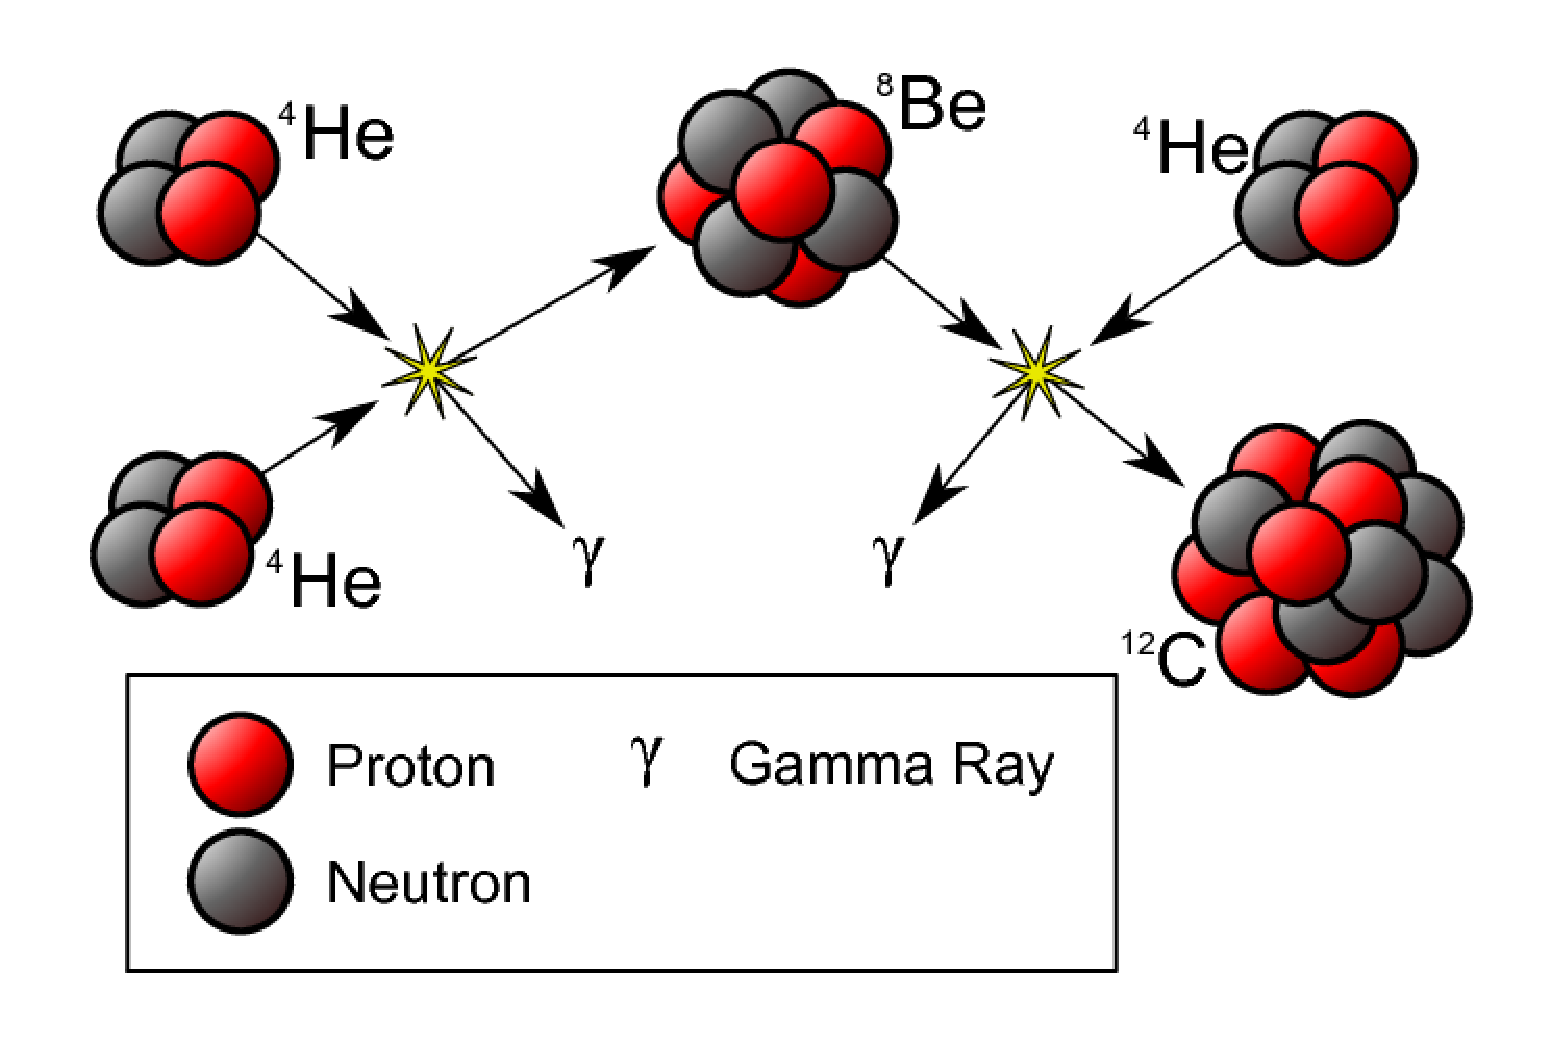
\includegraphics[scale=0.12]{media/triple-alpha_Wiki.pdf}
\end{columns}
Og med
\[
\varepsilon_{3\alpha}=\varepsilon_{0,3\alpha}\rho^2X_{He}^3T_8^{41}.
\]
hvor
\[
\varepsilon_{0,3\alpha}=3.86\times10^{-18}{\rm\ Wm^6/kg^3}
\]
Denne er gyldig omkring $T_8\approx1$.
\end{block}
\hyperlink{reak8}{\pagebutton{Neste side}}
\end{frame}



\begin{frame}
\label{reak8}
\lastpagebutton{reak7}{\bf SIDE 34/38/47}\\
{\Large
La du nok en gang merke til den temperaturavhengigheten eller???
\[
\varepsilon_{3\alpha}=\varepsilon_{0,3\alpha}\rho^2X_{He}^3T_8^{41}.
\]
Altså $T_6^{41}$ i \textcolor{red}{\Large\bf enogførtiende potens!!!!}. En virkelig \textcolor{red}{\bf\Huge ekstrem} temperaturavhengighet. Her ser vi at bittesmå endringer i temperatur vil ha utrolig stor effekt på energiproduksjonen og dermed luminositeten til stjerna.
Anta at kjernetemperaturen i en stjerne går fra 90 millioner grader til 110 millioner grader. Anta også at 3$\alpha$-prosess er eneste prosess som produserer energi. {\bf Hvor mye øker lumimnositeten til stjerna?} Du bør gjøre regningen så du får prøvd deg på å bruke uttrykket, mange sliter med dette!
}
\hyperlink{feil_reak8f}{\choicebutton{til det dobbelte}}\ \ \hyperlink{feil_reak8f}{\choicebutton{10 ganger}}\ \ \hyperlink{feil_reak8f}{\choicebutton{100 ganger}}\ \ \hyperlink{feil_reak8f}{\choicebutton{1000 ganger}}\ \ \hyperlink{riktig_reak8r}{\choicebutton{mer enn 1000 ganger}}\ \
\end{frame}

{
\setbeamercolor{background canvas}{bg=black}
\begin{frame}
\label{feil_reak8f}
\lastpagebutton{reak8}{\bf SIDE 35/38/47}\\
\textcolor{yellow}{\Large
Det ble galt. Du er klar over at 90 millioner Kelvin betyr $T_8=0.9$? Prøv igjen, og spør hvis du ikke får det rett!
}
\end{frame}
}


{
\setbeamercolor{background canvas}{bg=yellow}
\begin{frame}
\label{riktig_reak8r}
\clastpagebutton{reak8}{\bf SIDE 36/38/47}\\
{\Huge
Det ble riktig. Nærmere bestemt 3700 ganger så stor luminositet ved en temperaturøkning på omkring 20\%!!!!! En utrolig sensitiv reaksjon.
}
\hyperlink{reak9}{\pagebutton{Neste side}}
\end{frame}
}


\begin{frame}
\label{reak9}
\lastpagebutton{riktig_reak8r}{\bf SIDE 37/38/47}\\
{\bf La oss prøve å bruke dette på oppgave 6 fra avsluttende eksamen 2012:}
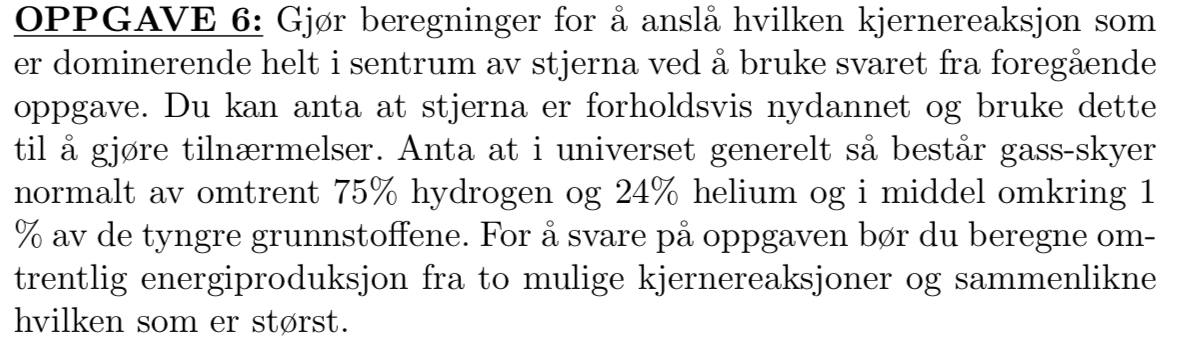
\includegraphics[scale=0.6]{media/eksamen2012_6.png}
{\small
Anta at massen til stjerna er $3M_\odot$, radien til stjerna er $1.2\times10^6$\,km og kjernetemperaturemn er 17 millioner Kelvin. Anta at massetettheten til stjerna er uniform (den samme gjennom hele) og at radien til kjernen til stjerna (den delen som har kjernereaksjoner) er $10\%$ av radien til stjerna. I tillegg til å finne hvilken prosess som er mest dominerende, finn også ut den totale luminositeten til stjerna, summert over pp-kjeden og CNO-syklusen. {\bf Prøv nå så godt du kan å få til dette selv!} Du må gå et par sider tilbake for å få tak i de riktige uttrykkene som du trenger.\\
}
\hyperlink{reak10}{\pagebutton{Jeg har forsøkt!}}
\end{frame}

\begin{frame}
\label{reak10}
\lastpagebutton{reak9}{\bf SIDE 38/38/47}\\
\begin{itemize}
\item Fikk du at pp-kjeden dominerer og produserer omtrent dobbelt så mye energi som CNO-syklusen?
\item Fikk du at total luminositet er omkring $4\times10^{23}$W (mens pp-kjeden gir opphav til en tredjedel av denne)
\end{itemize}
Hvis ikke, \href{https://www.uio.no/studier/emner/matnat/astro/AST2000/h20/undervisningsmateriell/interaktive-forelesningsnotater/3c/videoer/video3c_3.mp4}{ta en titt på denne videoen der du får noen hint}. Hvis hintene i videoen ikke var nok, snakke med gruppelærer!
{\bf MERK at resultatet du får her er urealistisk. En stjerne med 3 ganger solens masse, skal ha mye større luminositet en solen. Resultatet du fikk her svarer bare til 1/1000 solluminositet.} Tetthet og temperatur varierer selvfølgelig kraftig i forskjellig avstand fra kjernen. Uniform temperatur og tetthet er veldig urealistisk og verdiene som ble brukt her gir et urealistisk svar.
\hyperlink{blue_nytema4}{\pagebutton{Neste side}}
\end{frame}

\renewcommand{\headline}{Solnøytrinoproblemet}
{
\setbeamercolor{background canvas}{bg=blue}
\begin{frame}
\label{blue_nytema4}
\hyperlink{reak9}{\pagebutton{\small Forrige side}}
\nytemaside{0}
\hyperlink{snp1}{\pagebutton{Sett igang!}}
\end{frame}
}



\begin{frame}
\label{snp1}
\lastpagebutton{reak10}\label{snp}{\bf SIDE 39/47/47}\\
{\Large
Men er det ikke et vitenskaplig problem med det som vi nå holder på med? {\bf Altså:} vi har teorier for hvilke kjernereaksjoner som foregår inne i sentrum av en stjerne. {\bf Men skal en teori være vitenskaplig bør den vel testes?} Er det ikke det som er definisjonen av en vitenskaplig teori?? \textcolor{red}{Hvis vi aldri kommer inn under overflaten til en stjerne, kan vi aldri vite om teoriene våre er riktige, eller?} Dermed blir teorier for kjernereaksjonene i sentrum av en stjerne aldri ekte vitenskap?
}
\hyperlink{snp2}{\pagebutton{Yupp, dette blir bare noe kvasivitenskaplig tøv!}}
\end{frame}

\begin{frame}
\label{snp2}
\lastpagebutton{snp1}{\bf SIDE 40/47/47}\\
{\Large
{\bf ELLER?} Kan du ta en kikk til på disse kjernereaksjonene igjen? Her har du pp-kjeden igjen som er den som er aktuell for sola:\\
\begin{columns}
\column{0.7\textwidth}
\bua
{\hydrogen}+\hydrogen&\rightarrow&{\deuterium}+\positron+\neutrino \\
{\deuterium} +\hydrogen&\rightarrow&{\hethree}+\photon \\
{\hethree} +\hethree&\rightarrow&{\helium}+2\times\hydrogen
\eua
\column{0.3\textwidth}
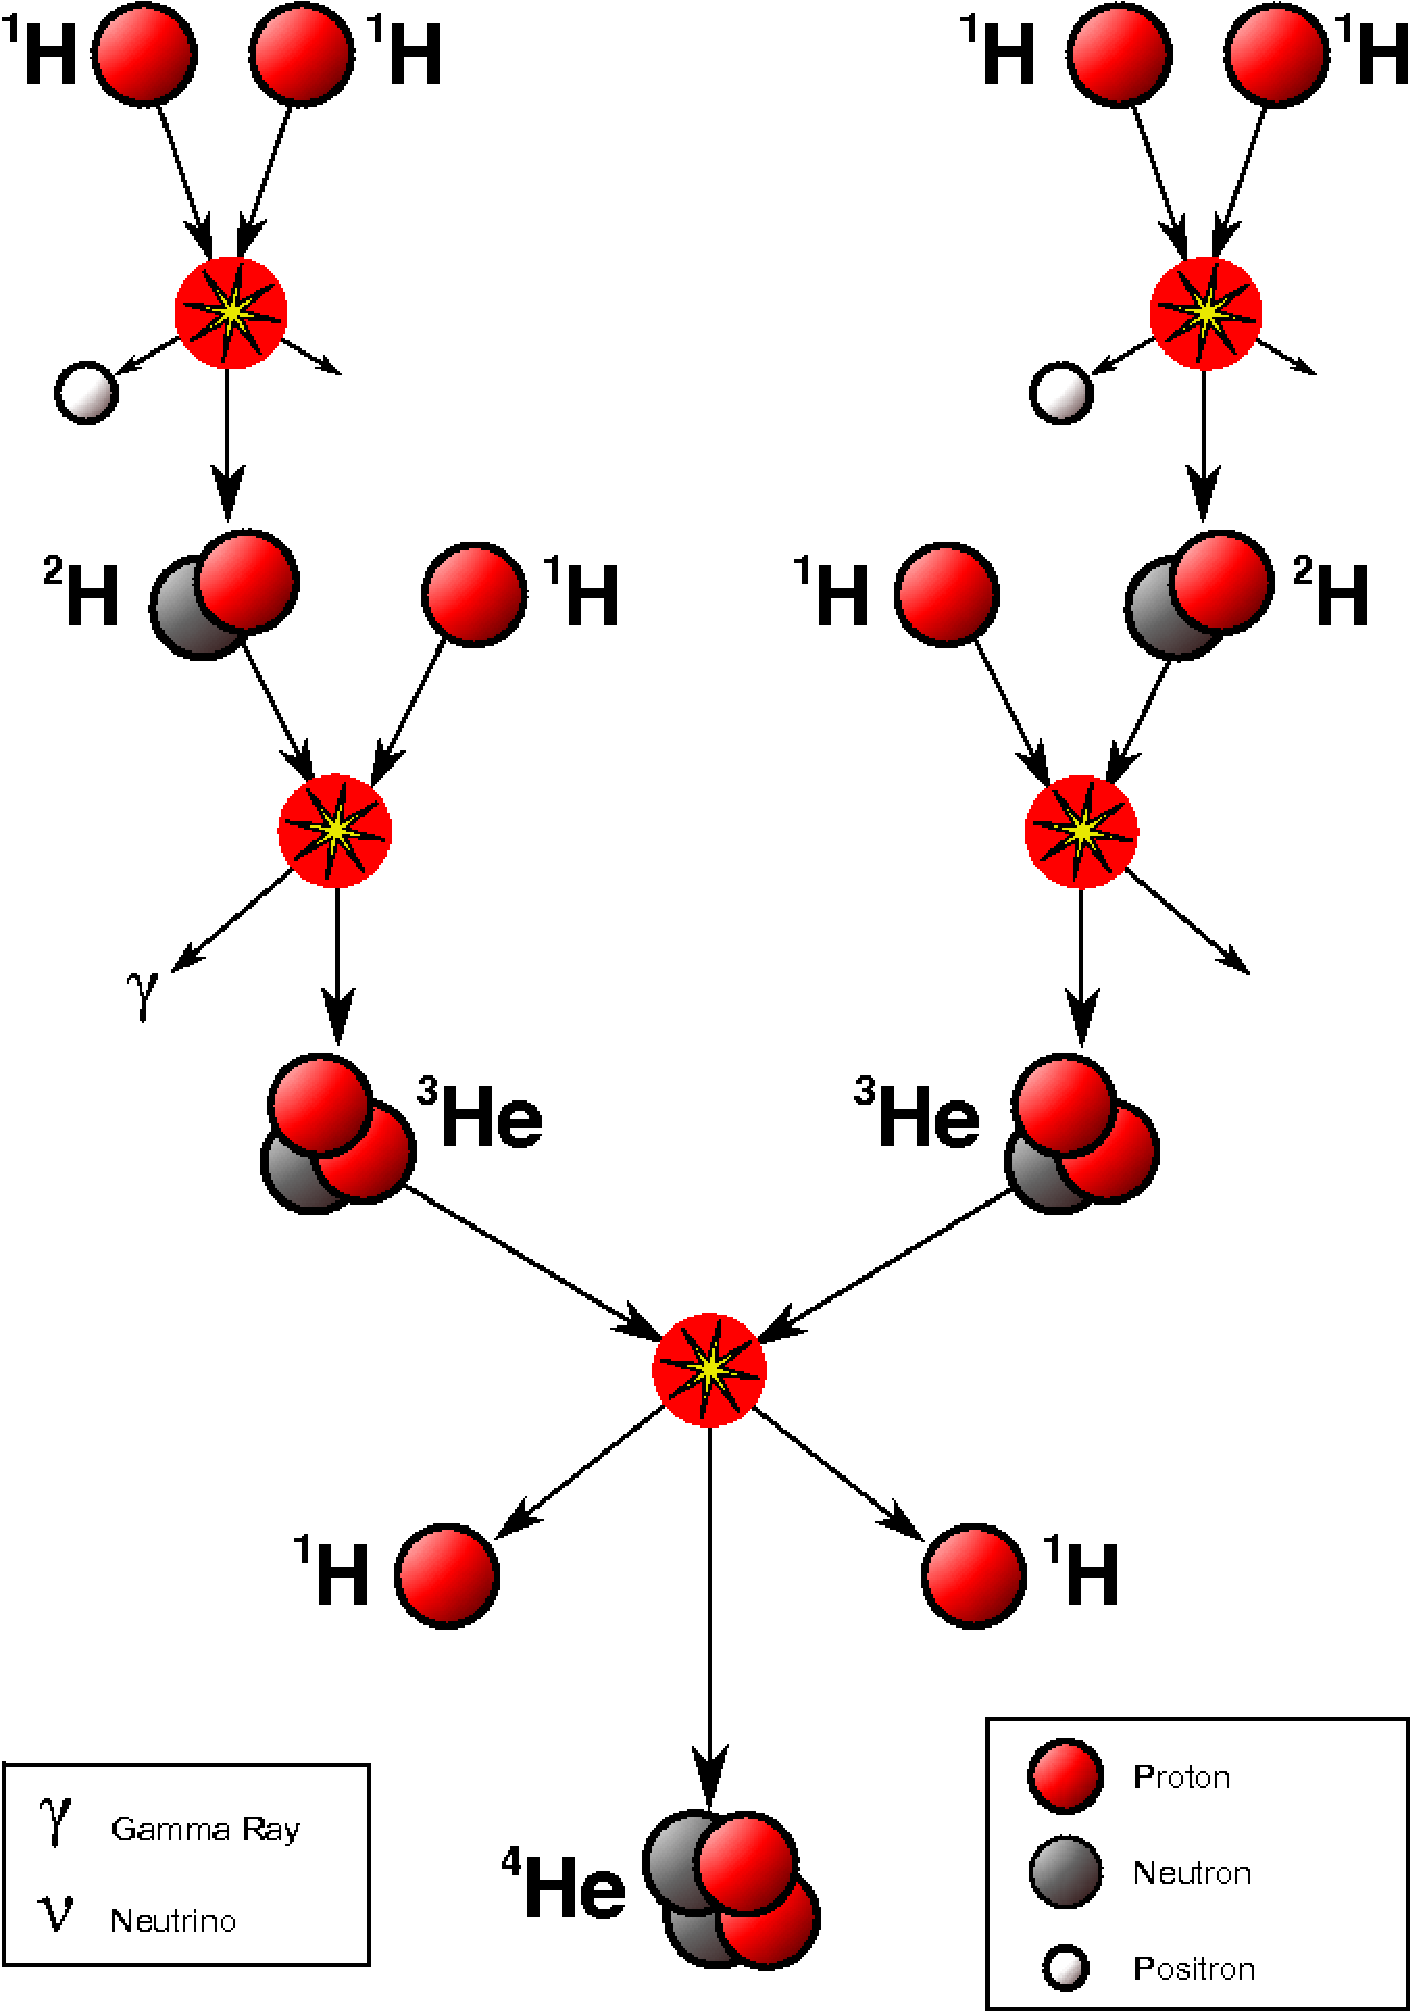
\includegraphics[scale=0.1]{media/pp_chain_Wiki.pdf}
\end{columns}
\textcolor{red}{Kan du se noe her som vi kunne bruke til å teste teoriene om kjernereaksjoner i sentrum av en stjerne?}
}
\hyperlink{snp3}{\pagebutton{Driver enda og tenker litt på det her...}}
\end{frame}

\begin{frame}
\label{snp3}
\lastpagebutton{snp2}{\bf SIDE 41/47/47}\\
{\Large
{\bf Ser du at det dannes nøytrinoer i denne reaksjonen?}
\begin{columns}
\column{0.7\textwidth}
\bua
{\hydrogen}+\hydrogen&\rightarrow&{\deuterium}+\positron+\neutrino \\
{\deuterium} +\hydrogen&\rightarrow&{\hethree}+\photon \\
{\hethree} +\hethree&\rightarrow&{\helium}+2\times\hydrogen
\eua
\column{0.3\textwidth}
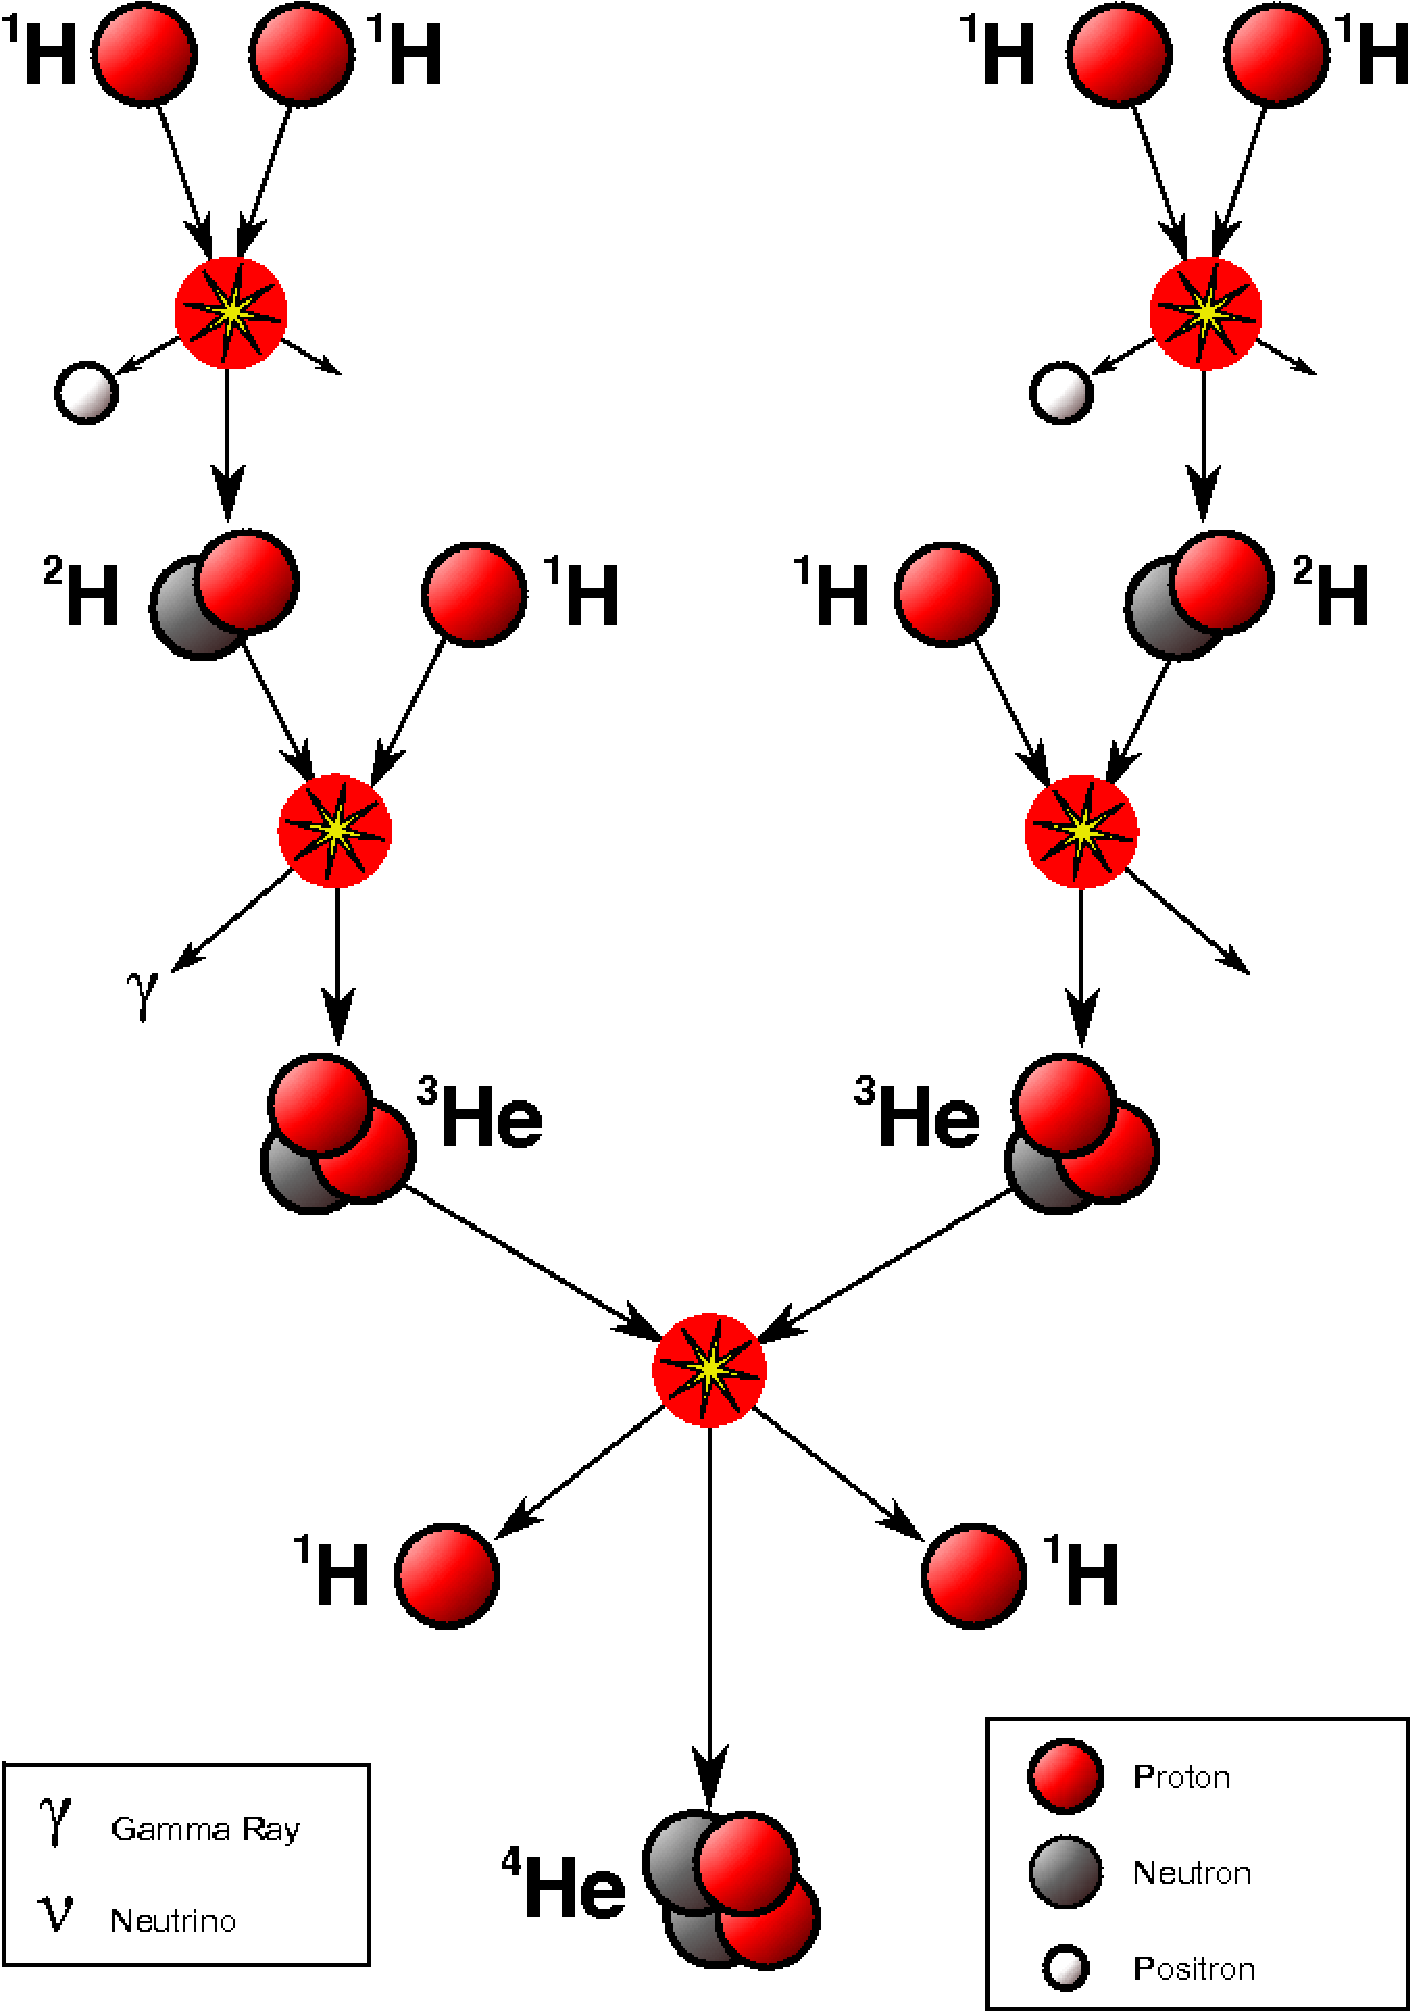
\includegraphics[scale=0.1]{media/pp_chain_Wiki.pdf}
\end{columns}
Var ikke nøytrinoene disse spøkelsespartiklene som bare går rett gjennom alt? (detektorer også) Og som i tillegg kunne virke som WDM (Warm Dark Matter) fordi de går med nær lysets hastighet? {\bf Hva har de med saken å gjøre? Kan de på noen måte gjøre teorien direkte testbar?}
}
\hyperlink{snp4}{\pagebutton{Driver enda og tenker litt på det her...}}
\end{frame}

\begin{frame}
\label{snp4}
\lastpagebutton{snp3}{\bf SIDE 42/47/47}\\
{\Large
Disse nøytrinoene vil jo stråle ut fra kjernen av sola og i alle mulige retninger, akkurat som lyset fra sola. {\bf Men siden de trenger gjennom alt så går de rett fra sentrum av sola og frem til oss!} Hadde vi hatt et nøytrinoteleskop så kunne vi altså tatt bilde av kjernereaksjonene i solens kjerne! \\
\vspace*{1cm}
{\bf Nå har vi ikke et ``nøytrinoteleskop'' men nøytrinodetektorer som detekterer nøytrinoer fra sola}. Modellene våre kan forutsi nøyaktig hvor mange nøytrinoer vi forventer fra sola, og så kan vi teste mot de vi mottar i detektorene!
}
\hyperlink{snp5}{\pagebutton{GENIALT! Og... har man resultater? Var det bare tøv?}}
\end{frame}


\begin{frame}
\label{snp5}
\lastpagebutton{snp4}{\bf SIDE 43/47/47}\\
Før vi skal avsløre hvordan det gikk, la oss først ta en titt på den vitenskaplige fremgangsmåten her:
\begin{enumerate}
\item Løs likningene for stjernemodellering, altså det koblede lingningsettet av differensial-likninger med hydrostatisk likevekt, luminositet per skall pluss div. likninger fra fluid-dynamikk og termodynamikk og få ute en modell med bl.a. $\rho(r)$ og $T(r)$ samt sammensetninger som funksjon av $r$ (avstand fra sentrum av stjerna)
\item Fra tetthet og temperatur, kan vi bruke likningene for kjernereaksjoner som vi har snakket om her til å regne ut nøyaktig hvor mange nøytrinoer som produseres som funksjon av $r$, og dermed det totale antall nøytrinoer for forskjellige energiområder $E$ som sendes ut fra en stjerne, i dette tilfellet sola, per sekund
\item Bruke nøytrinodetektorer til å måle fluksen av nøytrinoer på jorda i forskjellige energiband $E$ og sammenlikne med forutsigelsen i (2)
\item Hvis det er uoverensstemmelse, så gå tilbake til (1) og juster modellen basert på dataene. Får man til slutt en modell som gir riktig radius, overflatetemperatur of nøytrinofluks fra sola?
\end{enumerate}
\hyperlink{snp6}{\pagebutton{Javel, javel, men resultatene da? Stemte det?}}
\end{frame}

\begin{frame}
\label{snp6}
\lastpagebutton{snp5}{\bf SIDE 44/47/47}\\
{\Large I et par tiår så var svaret på dette spørsmålet \textcolor{red}{\Huge NEI!}}
\hyperlink{snp7}{\pagebutton{Ante meg, bare tøv hele greia!}}
\end{frame}



\begin{frame}
\label{snp7}
\lastpagebutton{snp6}{\bf SIDE 45/47/47}\\
{\Large Det som var litt rart var at uansett hva man gjorde så observerte man kun 1/3 av det antall nøytrinoer som modellene forutsa!|}
\hyperlink{snp8}{\pagebutton{Bare 1/3? Teoriene er altså helt på jorde ja!}}
\end{frame}


\begin{frame}
\label{snp8}
\lastpagebutton{snp7}{\bf SIDE 46/47/47}\\
MEN, man hadde gjort en gal antakelse! Man trodde på den tiden at nøytrinoene var massløse. Siden de er så vanskelige å detektere er de også notorisk vanskelige å måle massen til. Det virket som de beveget seg med noe nær lyshastighet, så man trodde at disse var masseløse som fotonene og dermed beveget seg med lyshastighet. {\bf MEN, standardmodellen i partikkelfysikk hadde en mulig variant: hvis nøytrinoene har masse, så vil de også hele tiden fluktuere mellom de forskjellige typene nøytrinoer. Husker du at det finnes 3 typer? Elektron-, myon og tauassosierte nøytrinoer. Hvis nøytrinoer har masse, så sier standardmodellen i partikkelfysikk at disse hele tiden spontant vil skifte mellom disse 3 typene}.\textcolor{red}{Nøytrinodetektorene man brukte den gangen registrerte kun elektron-nøytrinoer som jo er det som dannes i kjernereaksjonene.{\bf MEN hvis disse nå svinger mellom de forskjellige typene nøytrinoer på veien til oss, så vil vi kun motta 1/3 av disse som elektronnøytrinoer.}} Kunne denne 1/3 komme derfra? Var det rett og slett at de andre 2/3 an nøytrinoene hadde forvandlet seg til myon- og taunøytrinoer? {\bf (snakk om spøkelsespartikler ja!)}.
\hyperlink{snp9}{\pagebutton{Nå ble jeg spent her...}}
\end{frame}


\begin{frame}
\label{snp9}
\lastpagebutton{snp8}{\bf SIDE 47/47/47}\\
{\Large
De siste årene har man fått nøytrinodetektorer som detekterer alle typene nøytrinoer, og {\bf nå passer observasjonene helt med modellene!}. Og med på kjøpet så har det altså blitt slått fast at nøytrinoene ikke er masseløse partikler, de har masse og kan derfor svinge mellom de forskjellige typene!
}
\hyperlink{oppsummering}{\pagebutton{\small WOW, jeg er målløs! Dette var skikkelig vitenskaplig detektivarbeid!}}
\end{frame}


\begin{frame}
\label{oppsummering}
\hyperlink{snp9}{\pagebutton{\small Forrige side}}\href{https://nettskjema.no/a/167466}{\Changey[1][yellow]{2} \Changey[1][yellow]{-2}}
Gratulerer, del 3C er overstått. Du bør nå:
\begin{itemize}
\item vite hvorfor energi frigjøres i visse kjernereaksjoner
\item vite hvilke atomkjerner vi kan fusjonere og hvilke vi kan fisjonere for å få energi
\item hvordan atomkjerner kan overvinne Columbkrafta og få til fusjon
\item vite hva $\epsilon$ er og hvordan den kan brukes til å finne uttrykket for luminositet fra et skall i en stjerne
\item kunne regne ut luminositeten til en stjerne basert på kjernereaksjonene i stjerna
\item vite hva solnøytrinoproblemet var og hvordan det ble løst
\end{itemize}
\textcolor{red}{Flott hvis du nå kan klikke på smilefjesene over og fortelle hva du synes om dette interaktive forelesningsnotatet. Hva var bra og nøyaktig hva kan forbedres? All ris og ros mottaes med takk!}
{\bf Det anbefales nå at du sjekker \href{https://www.uio.no/studier/emner/matnat/astro/AST2000/h21/undervisningsmateriell/kortsvarsoppgaver/del3c.pdf}{kortsvarsoppgavene} til del 3C for å kontrollere at du har forstått stoffet. Kan du svare på disse, blir det lettere å bruke kunnskapen din i oppgavene/prosjektet. Noen av disse kommer på eksamen.}
\end{frame}



\end{document}
